% LaTeX Präsentationsvorlage (2013) der TU Graz, rev12, 2013/01/31
\documentclass{beamer}
%\documentclass[aspectratio=169]{beamer}
% \usetheme{tugraz2013}
% \usetheme[notes]{tugraz2013}
\usetheme[minimal]{tugraz2013}
\usepackage[utf8]{inputenc}
\usepackage[american]{babel}
\usepackage{color, colortbl}
\usepackage{listings}
\usepackage{tikz}
\usepackage{alltt}

\usepackage{amssymb}% http://ctan.org/pkg/amssymb
\usepackage{pifont}% http://ctan.org/pkg/pifont
\newcommand{\cmark}{\ding{51}}%
\newcommand{\xmark}{\ding{55}}%

%\usepackage{ulem}
\usetikzlibrary{calc,trees,positioning,arrows,chains,shapes.geometric,decorations.pathreplacing,decorations.pathmorphing,shapes,matrix,shapes.symbols}
%\newcommand{\iocosymbol}{\ensuremath{\mbox{\it{ioco}}}\xspace}
\makeatletter
\def\cellcolor{{\ifnum0=`}\fi\bmr@cellcolor}
\newcommand<>{\bmr@cellcolor}{%
    \alt#1%
        {\global\let\CT@do@color\CT@@do@color\@ifnextchar[\CT@rowa\CT@rowb}% 
        {\ifnum0=`{\fi}\@gooble@cellcolor}% 
}

\newcommand{\@gooble@cellcolor}[2][]{\@gooble@cellcolor@}
\newcommand{\@gooble@cellcolor@}[1][]{\@gooble@cellcolor@@}
\newcommand{\@gooble@cellcolor@@}[1][]{\ignorespaces}
\makeatother

% This sets a new round of anchors at a specified multiple of the current ones
\def\pgf@sh@@knotanchor#1#2{%
  \anchor{#2 north west}{%
    \csname pgf@anchor@knot #1@north west\endcsname%
    \pgf@x=#2\pgf@x%
    \pgf@y=#2\pgf@y%
  }%
  \anchor{#2 north east}{%
    \csname pgf@anchor@knot #1@north east\endcsname%
    \pgf@x=#2\pgf@x%
    \pgf@y=#2\pgf@y%
  }%
  \anchor{#2 south west}{%
    \csname pgf@anchor@knot #1@south west\endcsname%
    \pgf@x=#2\pgf@x%
    \pgf@y=#2\pgf@y%
  }%
  \anchor{#2 south east}{%
    \csname pgf@anchor@knot #1@south east\endcsname%
    \pgf@x=#2\pgf@x%
    \pgf@y=#2\pgf@y%
  }%
  \anchor{#2 north}{%
    \csname pgf@anchor@knot #1@north\endcsname%
    \pgf@x=#2\pgf@x%
    \pgf@y=#2\pgf@y%
  }%
  \anchor{#2 east}{%
    \csname pgf@anchor@knot #1@east\endcsname%
    \pgf@x=#2\pgf@x%
    \pgf@y=#2\pgf@y%
  }%
  \anchor{#2 west}{%
    \csname pgf@anchor@knot #1@west\endcsname%
    \pgf@x=#2\pgf@x%
    \pgf@y=#2\pgf@y%
  }%
  \anchor{#2 south}{%
    \csname pgf@anchor@knot #1@south\endcsname%
    \pgf@x=#2\pgf@x%
    \pgf@y=#2\pgf@y%
  }%
}
% this defines the new node shape, inheriting most from the circle shape
\pgfdeclareshape{knot crossing}
{
  \inheritsavedanchors[from=circle] % this is nearly a circle
  \inheritanchorborder[from=circle]
  \inheritanchor[from=circle]{north}
  \inheritanchor[from=circle]{north west}
  \inheritanchor[from=circle]{north east}
  \inheritanchor[from=circle]{center}
  \inheritanchor[from=circle]{west}
  \inheritanchor[from=circle]{east}
  \inheritanchor[from=circle]{mid}
  \inheritanchor[from=circle]{mid west}
  \inheritanchor[from=circle]{mid east}
  \inheritanchor[from=circle]{base}
  \inheritanchor[from=circle]{base west}
  \inheritanchor[from=circle]{base east}
  \inheritanchor[from=circle]{south}
  \inheritanchor[from=circle]{south west}
  \inheritanchor[from=circle]{south east}
  \inheritanchorborder[from=circle]
  \pgf@sh@@knotanchor{crossing}{2}
  \pgf@sh@@knotanchor{crossing}{3}
  \pgf@sh@@knotanchor{crossing}{4}
  \pgf@sh@@knotanchor{crossing}{8}
  \pgf@sh@@knotanchor{crossing}{16}
  \pgf@sh@@knotanchor{crossing}{32}
  \backgroundpath{
    \pgfutil@tempdima=\radius%
    \pgfmathsetlength{\pgf@xb}{\pgfkeysvalueof{/pgf/outer xsep}}%
    \pgfmathsetlength{\pgf@yb}{\pgfkeysvalueof{/pgf/outer ysep}}%
    \ifdim\pgf@xb<\pgf@yb%
      \advance\pgfutil@tempdima by-\pgf@yb%
    \else%
      \advance\pgfutil@tempdima by-\pgf@xb%
    \fi%
  }
}



\lstdefinelanguage{ooa} {
  alsoletter={ ; , [] , |[ , ]|, 0, 1, 2, 3, 4, 5, 6, 7, 8, 9 },
  morekeywords={types, methods, do, obs, action, end, ctr, requires, od},
  morekeywords={signal, after, actions, var},
  morekeywords={|[, ]|, ; , [], public, autocons, system},
   emph={SmallInt, TimeSteps, int, Int, bool, AlarmSystem},
   emphstyle=\color{brown},
%   emph={true, false, and, not, of, len, //, hd, tl },
%   emphstyle=\color{black},
%   emph={ ; , [] },
%   emphstyle=\color{red},
   sensitive=true,
%   morecomment=[s]{/*}{*/},
   comment=[l]{\#},
   showspaces=false,
   showstringspaces=false,
   numbers=left,
   numbersep=5pt,
   numberstyle=\tiny,
%   showtabs=true,
   tabsize=2,
   escapeinside={@}{@},
   framexleftmargin=9pt,
  }





%% Titelblatt-Einstellungen
\title[Formal Test-Driven Development with Verified Test Cases]{Formal Test-Driven Development
with Verified Test Cases}
\author{Bernhard K. Aichernig\textsuperscript{1}, Florian Lorber\textsuperscript{1}, and \underline{Stefan Tiran}\textsuperscript{1,2}}
%\today
% \date{Graz, XX. Dezember 2010}		% \today für heutiges Datum verwenden
%\date{\today}
\date{Lisbon, 2014-01-09}
%\date{Graz, 2013-06-20}		% \today für heutiges Datum verwenden

% \institutelogo{kurz.pdf}
%\additionallogo{institutslogo.pdf}
\institute[TU Graz / AIT]{\textsuperscript{1}Graz,~University of Technology \textsuperscript{2}Austrian Insitute of Technology}
\instituteurl{www.tugraz.at}
% \institutelogo{kurz.pdf}
%\additionallogo{institutslogo.pdf}
\additionallogo{ait_logo.jpg}
\additionallogoB{mbat_logo-light-crop.pdf}

%%%%%%%%%%%%%%%%%%%%%%%%%%%%%%%%%%%%%%%%%%%%%%%%%%%%%%%%%%%%%%%%%%%%%%%%%%%%
\begin{document}
%%%%%%%%%%%%%%%%%%%%%%%%%%%%%%%%%%%%%%%%%%%%%%%%%%%%%%%%%%%%%%%%%%%%%%%%%%%%
\titleframe

\begin{frame}
  \frametitle{Agenda}
%  My presentation is structured as follows: \ldots
  \begin{itemize}
    \item Motivation
    \item Running example: a car alarm system
    \item A formal test-driven development process
    \item Three iterations
    \begin{itemize}
      \item Model
      \item Test case generation
      \item Verification of test cases
      \item Results
    \end{itemize}
    \item Discussion / Conclusion
  \end{itemize}

\end{frame}

%\begin{frame}
%  \frametitle{Overview}
%  \tableofcontents%[hideallsubsections] 
%  \note{
%  	My presentation is structured as follows: \ldots
%  }
%\end{frame}

%\section{Introduction to Model-Based (Mutation) Testing}




% \section{Partial Models and Underspecification}
% \begin{frame}
%   \frametitle{Partial Models and Underspecification}
%   \begin{itemize}
%     \item Idea: Split test model into functional components (horizontal modularity)
%     \item Leave other parts underspecified
%     \item Combination of partial models is kind of refinement (vertical modularity)
%   \end{itemize}
% \end{frame}
% \section{Test-Driven Development}
% \begin{frame}
%   \frametitle{Test-Driven Development}
%   \begin{itemize}
%     \item Test-driven development made popular by Kent Beck
%     \item Classical:
%     \begin{itemize}
%       \item Start development of system by writing test cases
%       \item Implement system until test cases pass
%     \end{itemize}
%     \item Using model-based mutation testing:
%     \begin{itemize}
%       \item Series of partial test models
%       \item Each iteration: either new functionality (horizontal modularity) or refinement (vertical modularity)
%     \end{itemize}
%   \end{itemize}
% \end{frame}

%%%%%%%%%%%%%%%%%%%%%%%%%%%%%%%%%%%%%%%%%%%%%%%%%%%%%%%%%%%%%%%%%%%%%%%%%%%%
\section{Development Process}
%%%%%%%%%%%%%%%%%%%%%%%%%%%%%%%%%%%%%%%%%%%%%%%%%%%%%%%%%%%%%%%%%%%%%%%%%%%%


\begin{frame}
  \frametitle{Development Process - The Idea}
\setbeamercovered{invisible}
%\begin{center}
\begin{minipage}[T]{0.5\textwidth}
  \resizebox{!}{0.7\textheight}{
  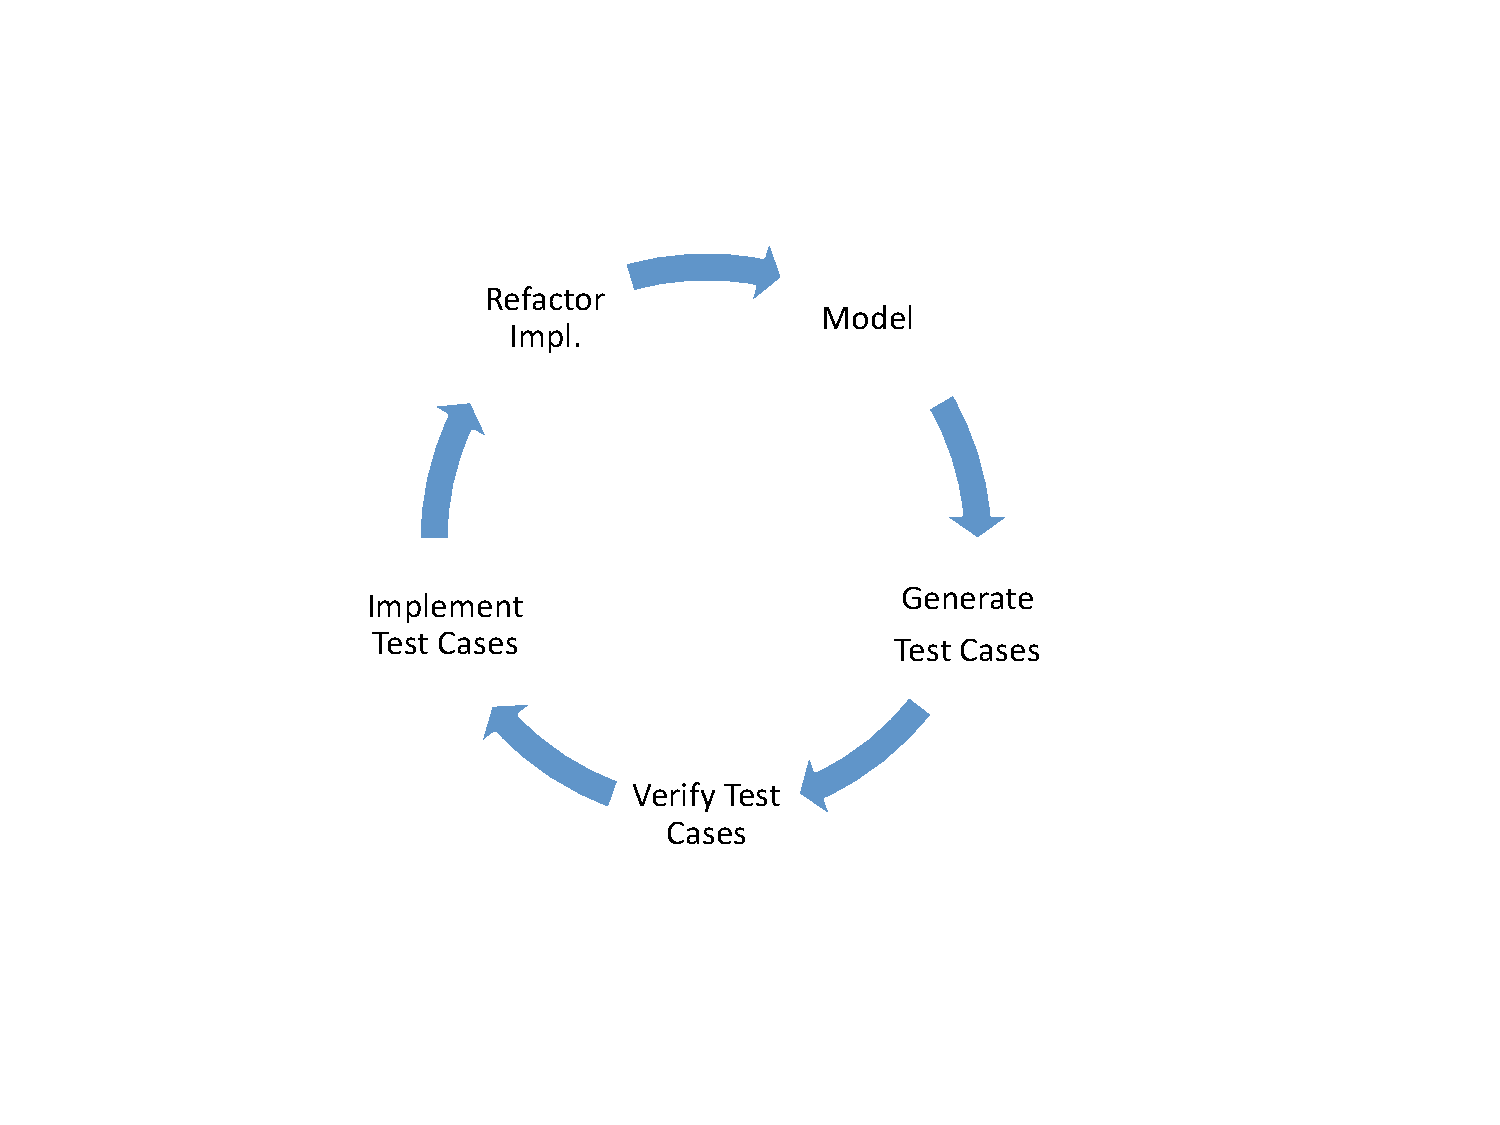
\includegraphics{figures/cycle}
}
\end{minipage}
\hspace{0.04\textwidth}
\begin{minipage}[T]{0.4\textwidth}
\vspace{-3.9cm}
  \resizebox{!}{0.4\textheight}{
    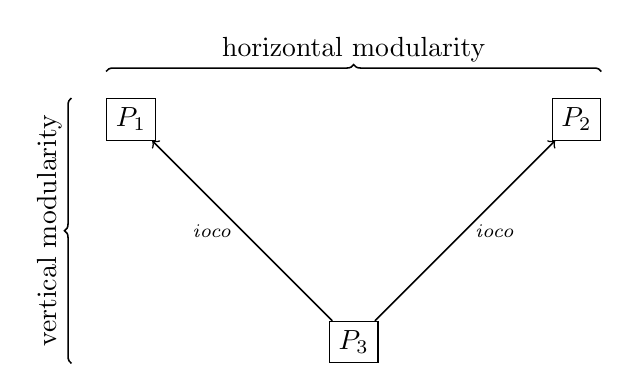
\begin{tikzpicture}[node distance=4cm]
      \tikzstyle{pm}=[rectangle,draw]
      \tikzstyle{br}=[decorate]
      \visible<4->{\node[pm] (P3) {$P_3$};} 
      \visible<2->{\node[pm] (P1) [above left of=P3] {$P_1$};}
      \visible<3->{\node[pm] (P2) [above right of=P3] {$P_2$};}

      \visible<4->{\draw[->,line width=.02cm] (P3) -- (P1) node[anchor=east, midway]{\scriptsize \textit{ioco}};}
      \visible<4->{\draw[->,line width=.02cm] (P3) -- (P2) node[anchor=west, midway]{\scriptsize \textit{ioco}};}
       \visible<3->{\draw[br,line width=.02cm][decoration={brace}] let \p1=(P1.south west), \p2=(P2.south east) in
      ($(\x1,\y1+2.5em)$) -- ($(\x2,\y2+2.5em)$) node[above,midway]
      {horizontal modularity};}
      \visible<4->{\draw[br,line width=.02cm][decoration={brace}] let \p2=(P1.north west), \p1=(P3.south west)
      in ($(\x2-1.25em,\y1)$) -- ($(\x2-1.25em,\y2)$)
      node[above,midway, rotate=90]
      {vertical modularity}; }
    \end{tikzpicture}
}
\end{minipage}
%\end{center}
\end{frame}
%%%%%%%%%%%%%%%%%%%%%%%%%%%%%%%%%%%%%%%%%%%%%%%%%%%%%%%%%%%%%%%%%%%%%%%%%%%%
\section{Motivation}
%%%%%%%%%%%%%%%%%%%%%%%%%%%%%%%%%%%%%%%%%%%%%%%%%%%%%%%%%%%%%%%%%%%%%%%%%%%%
\begin{frame}
  \frametitle{Motivation}
  \begin{itemize}
    \item Test cases play central role in software development
    \item Writing test cases is tedious
    \item Test cases need maintenance
    \item Model-based testing can help
    \begin{itemize}
      \item Test cases are generated automatically
      \item Models more stable to changes
      \item Abstract test cases less exposed to interface changes
    \end{itemize}
  \end{itemize}
\end{frame}

\begin{frame}
  \frametitle{Motivation cont.}
  \begin{itemize}
    \item Wrong models lead to wrong test cases
    \item Validation and verification needed
    \item Lack of model-checkers within model-based testing tools\\
    $\rightarrow$ validate test cases instead
  \end{itemize}
\end{frame}

\begin{frame}
  \frametitle{Motivation cont.}
  \begin{itemize}
    \item Test models need to evolve over time
    \item Idea: create series of partial test models
    \item Partial test models focus on functional components
    \item Partial test models can be refined into more detailed test models
    \item Support of conformance relation needed\\
    $\rightarrow$ Tretmans' ioco$^{*}$
  \end{itemize}
{\linespread{.05}\tiny* Jan Tretmans: Test Generation with Inputs, Outputs and Repetitive Quiescence. Software - Concepts and Tools 17(3): 103-120 (1996) }
\end{frame}



%%%%%%%%%%%%%%%%%%%%%%%%%%%%%%%%%%%%%%%%%%%%%%%%%%%%%%%%%%%%%%%%%%%%%%%%%%%%
\section{Running Example: Car Alarm System}
%%%%%%%%%%%%%%%%%%%%%%%%%%%%%%%%%%%%%%%%%%%%%%%%%%%%%%%%%%%%%%%%%%%%%%%%%%%%
\begin{frame}
  \frametitle{Running Example: Car Alarm System}
  \begin{itemize}
    \item Demonstrator within past {MOGENTES} project
    \item Requirements provided by Ford
    \item Default example of our workgroup
    \item Reuse of artifacts from former studies
    \begin{itemize}
      \item Java implementation (simulation)
      \item 38 faulty implementations from former experiments to measure quality of test suite
%      \item 8 handwritten test purposes
    \end{itemize}
  \end{itemize}
\end{frame}

\subsection{Core Requirements}
\begin{frame}
  \frametitle{Core Requirements}
  \begin{enumerate}
\item \textbf{Arming.} The system is armed 20 seconds
after the vehicle is locked and the bonnet, luggage compartment, and
all doors are closed.

\item \textbf{Alarm.} The alarm sounds for 30 seconds if
an unauthorized person opens the door, the luggage compartment, or the
bonnet. The hazard flasher lights will flash for five minutes.

\item \textbf{Deactivation.} The anti-theft alarm system
can be deactivated at any time, even when the alarm is sounding, by
unlocking the vehicle from outside.
  \end{enumerate}
\end{frame}



%%%%%%%%%%%%%%%%%%%%%%%%%%%%%%%%%%%%%%%%%%%%%%%%%%%%%%%%%%%%%%%%%%%%%%%%%%%%
\section{A Formal Test-Driven Development Process}
%%%%%%%%%%%%%%%%%%%%%%%%%%%%%%%%%%%%%%%%%%%%%%%%%%%%%%%%%%%%%%%%%%%%%%%%%%%%
\subsection{Initial Phase}
\begin{frame}
  \frametitle{Initial Phase}
  \begin{itemize}
    \item Define test interface for test models (inputs / outputs)
    \item Define test interface on implementation level (e.g. method calls)
    \item Implement test adapter / test driver
  \end{itemize}

\end{frame}
\begin{frame}
  \frametitle{Initial Phase cont.}
  Test interface of the car alarm system
  \begin{itemize}
    \item Controllable Actions (ctr): Close, Lock, Unlock, Open
    \item Observable Actions (obs): ArmedOn, ArmedOff, SoundOn, SoundOff, FlashOn, FlashOff
  \end{itemize}

\end{frame}


\defverbatim[colored]\Lsta{%
 \begin{lstlisting}[language=ooa,linewidth=\textwidth,breaklines,basicstyle=\scriptsize,keywordstyle=\bfseries\color{green!40!black},commentstyle=\itshape\color{purple!40!black},stringstyle=\color{orange}]
types
  TimeSteps = {I0 = 0, I20 = 20, I30 = 30, I270 = 270} ;
  Int = int[0..270] ;
  SmallInt = int[0..3] ;
  AlarmSystem = autocons system
  |[
    var
      open      : bool = true ;
      locked    : bool = false ;
      armed     : bool = false ;
      armedOn   : bool = false ;
      armedOff  : bool = false ;
      semaphore : Int  = 0
 \end{lstlisting}}

\defverbatim[colored]\Lstb{%
 \begin{lstlisting}[language=ooa,linewidth=\textwidth,breaklines,firstnumber=14,basicstyle=\scriptsize,keywordstyle=\bfseries\color{green!40!black},commentstyle=\itshape\color{purple!40!black},stringstyle=\color{orange}]
    actions
      ctr Close ( wtime : Int ) =
        requires not armed :
          requires open and wtime = 0 and semaphore = 0 and locked :
            open := false ;
            armedOn := true
          end 
          []
          requires open and wtime = 0 and semaphore = 0 and not locked :
            open := false 
            end
          end
       ;
 \end{lstlisting}}

\defverbatim[colored]\Lstc{%
 \begin{lstlisting}[language=ooa,linewidth=\textwidth,breaklines,firstnumber=27,basicstyle=\scriptsize,keywordstyle=\bfseries\color{green!40!black},commentstyle=\itshape\color{purple!40!black},stringstyle=\color{orange}]
      obs ArmedOn (wtime : Int) =
        requires (armedOn and wtime = 20):
          armedOn := false ;
          armed := true
          end
      ;
      obs ArmedOff (wtime : Int) =
        requires (armedOff and wtime = 0) :
          armedOff := false ;
          semaphore := semaphore - 1 ;
          armed := false
        end
 \end{lstlisting}}
\defverbatim[colored]\Lstd{%
  \begin{lstlisting}[language=ooa,linewidth=\textwidth,breaklines,firstnumber=39,basicstyle=\scriptsize,keywordstyle=\bfseries\color{green!40!black},commentstyle=\itshape\color{purple!40!black},stringstyle=\color{orange}]
    do
      var A : TimeSteps : Close (A)   [] 
      var B : TimeSteps : Open (B)    []
      var C : TimeSteps : Lock (C)    []
      var D : TimeSteps : Unlock (D)  []
      var E : TimeSteps : ArmedOn (E) []
      var F : TimeSteps : ArmedOff (F)        
    od
  ]|

system
  AlarmSystem
 \end{lstlisting}}

\subsection{Model}

\begin{frame}
  \frametitle{Modeling Approach}
  \begin{itemize}
    \item Object oriented adaption of Back's Action Systems$^{*}$
    \item Textual modeling language with precise semantics
    \item Translator for UML state machines exists
    \item Interpreted and transformed to Labeled Transition System
    \item Visualized using the CADP toolbox$^{**}$
  \end{itemize}
  {\linespread{.05}\tiny* Back, R.-J. and Kurki-Suonio, R. (1983). Decentralization
of process nets with centralized control. In 2nd ACM
SIGACT-SIGOPS Symp. on Principles of Distributed
Computing, pages 131–142. ACM.\\
** \url{http://www.inrialpes.fr/vasy/cadp/}
}

\end{frame}

\section{Iteration 1}
\subsection{The Model}
\begin{frame}
  \frametitle{Iteration 1 - The Model}
\begin{minipage}[T]{0.4\textwidth}
  \resizebox{!}{0.7\textheight}{
  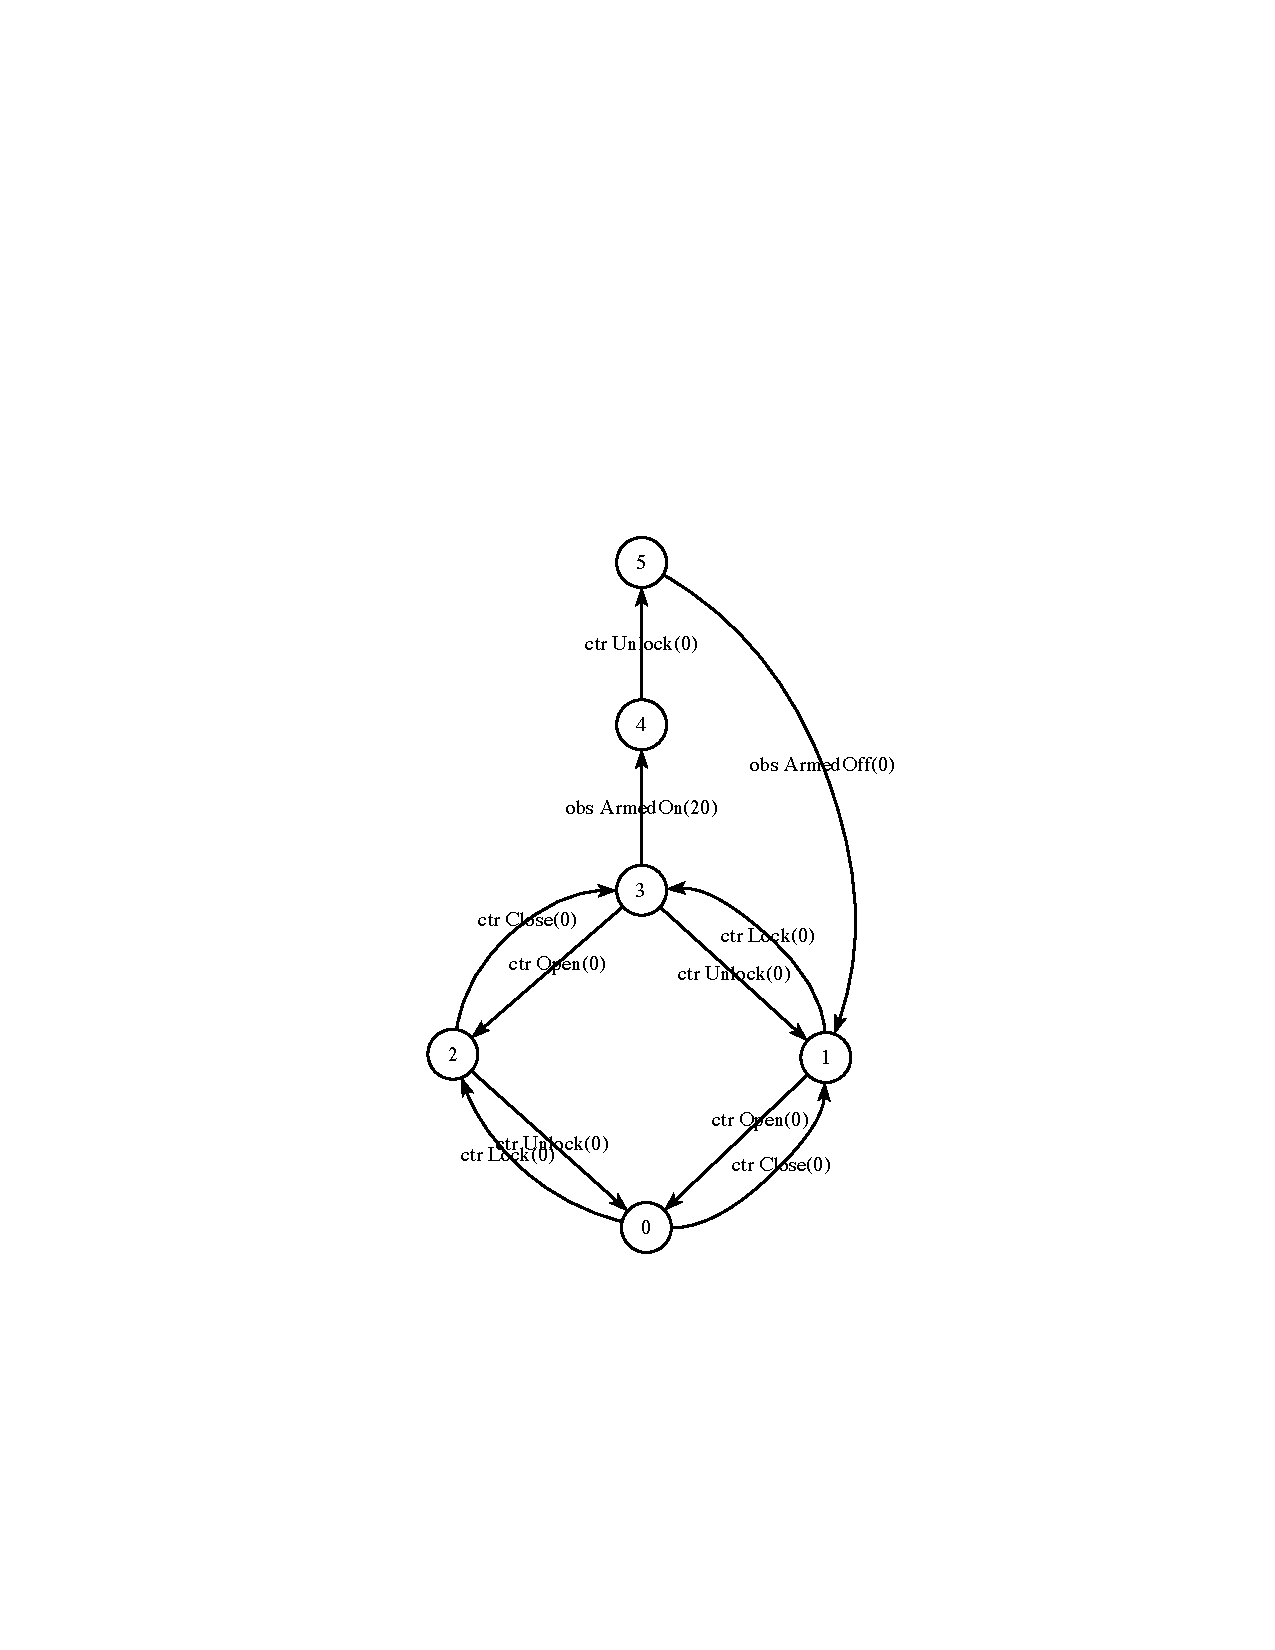
\includegraphics{figures/cas1}
}
\end{minipage}
\hspace{0.04\textwidth}
\begin{minipage}[T]{0.42\textwidth}{
  \begin{itemize}
    \item Labeled Transition System
    \item First partial model: $CAS_1$
    \item Arming and disarming behavior
  \end{itemize}
}
\end{minipage}
\end{frame}

\subsection{Generate Test Cases}
\begin{frame}
  \frametitle{Generate Test Cases}
%  \vspace{-.9cm}
%  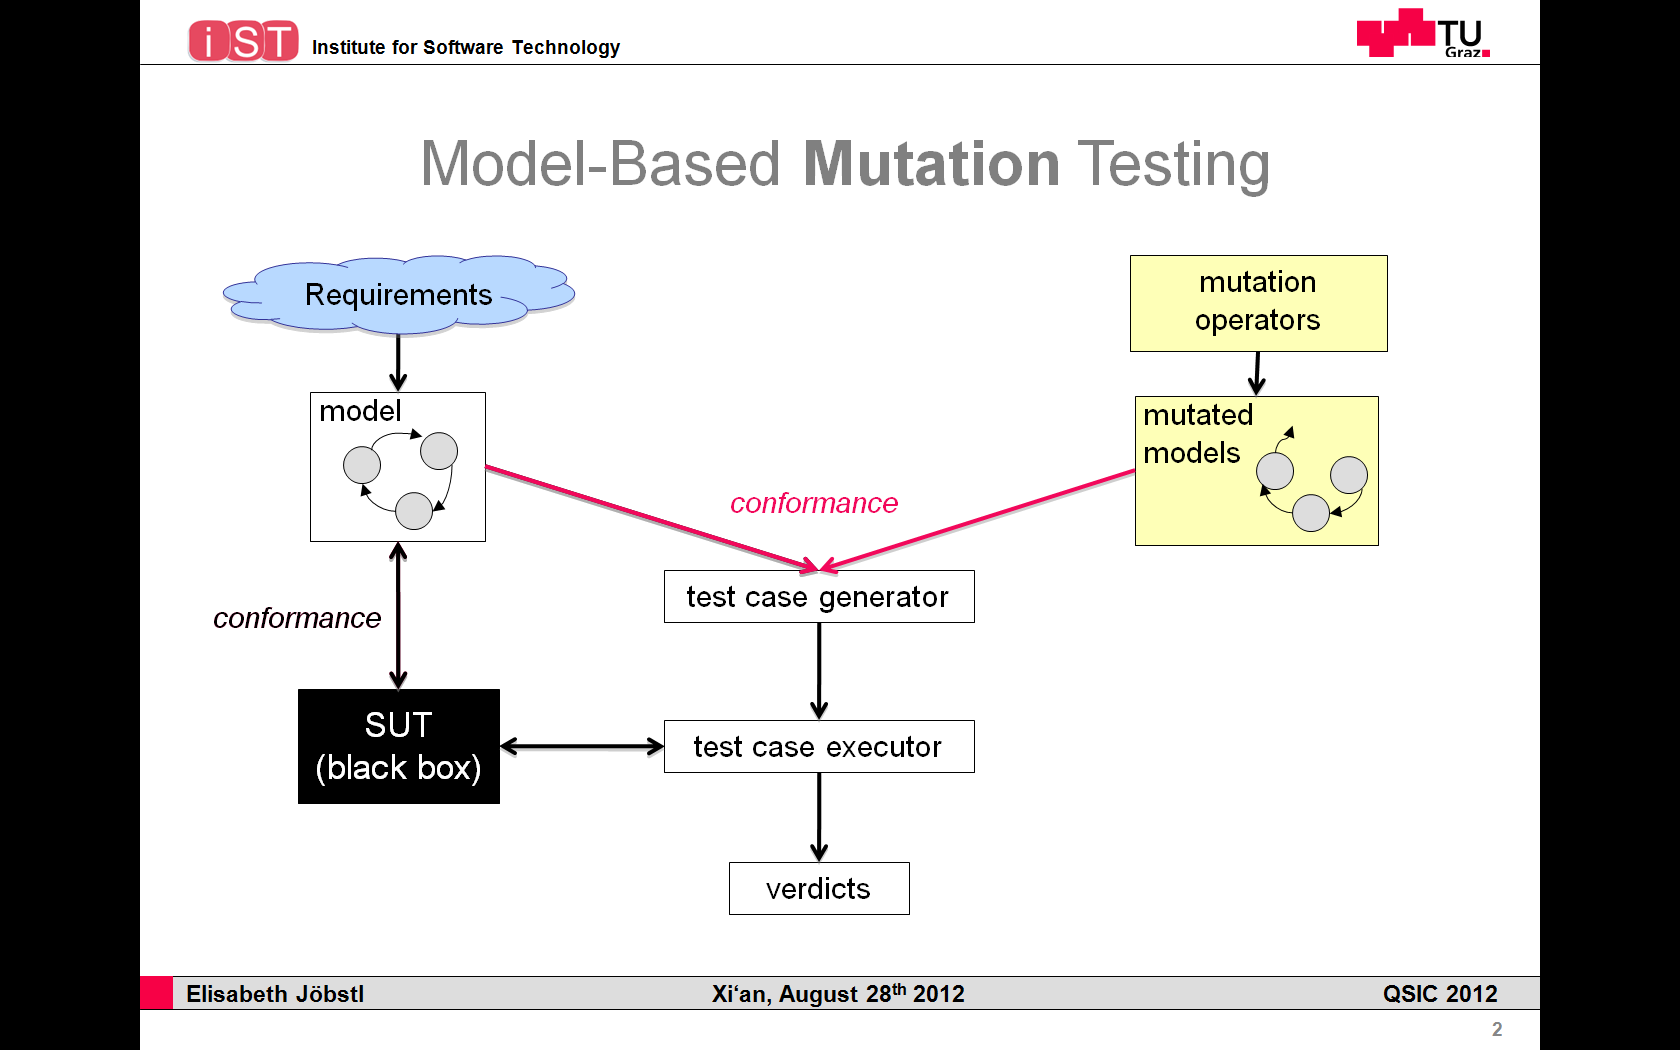
\includegraphics[width=\textwidth,trim=110 100 200 150, clip]{figures/MBMT}  

%  \resizebox{0.99\textwidth}{!}{\tiny Source: Bernhard K. Aichernig and Elisabeth Jöbstl: Efficient Refinement Checking for Model-Based Mutation Testing. Xi'an, August 2012}

    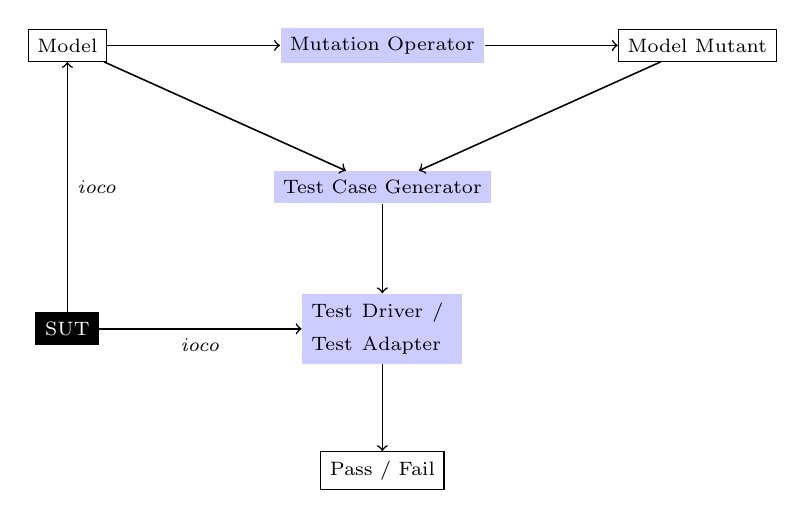
\begin{tikzpicture}[node distance=4cm]
      \tikzstyle{tool}=[rectangle,fill=blue!20!white]
      \tikzstyle{pm}=[rectangle,draw]
      \tikzstyle{br}=[decorate]
      \tikzstyle{blackbox}=[rectangle,draw,fill=black,text=white]
      \node[pm] (verdict) {\scriptsize Pass / Fail};
      \node[tool] (tdta) [node distance=1.8cm, above of=verdict, text width=1.8cm] {\scriptsize Test Driver / Test Adapter};
      \node[tool] (tcg) [node distance=1.8cm, above of=tdta] {\scriptsize Test Case Generator} ;
      \node[tool] (mutop) [node distance=1.8cm, above of=tcg] {\scriptsize Mutation Operator} ;
      \node[blackbox] (SUT) [left of=tdta] {\scriptsize SUT} ;
      \node[pm] (model) [left of=mutop] {\scriptsize Model} ;
      \node[pm] (mutant) [right of=mutop] {\scriptsize Model Mutant} ;

      \draw[->,line width=.02cm] (SUT) -- (tdta) node[anchor=north, midway]{\scriptsize \textit{ioco}};
      \draw[->,line width=.02cm] (SUT) -- (model) node[anchor=west, midway]{\scriptsize \textit{ioco}};
      \draw[->,line width=.02cm] (model) -- (tcg) node[anchor=west, midway]{};
      \draw[->,line width=.02cm] (model) -- (mutop) node[anchor=west, midway]{};
      \draw[->,line width=.02cm] (mutop) -- (mutant) node[anchor=west, midway]{};
      \draw[->,line width=.02cm] (mutant) -- (tcg) node[anchor=west, midway]{};
      \draw[->,line width=.02cm] (tcg) -- (tdta) {};
      \draw[->,line width=.02cm] (tdta) -- (verdict) {};

      % \draw[->] (P3) -- (P1) node[anchor=east, midway]{\textit{ioco}};
      % \draw[->] (P3) -- (P2) node[anchor=west, midway]{\textit{ioco}};
      % \draw[br][decoration={brace}] let \p1=(P1.south west), \p2=(P2.south east) in
      % ($(\x1,\y1+2.5em)$) -- ($(\x2,\y2+2.5em)$) node[above,midway]
      % {horizontal modularity};
      % \draw[br][decoration={brace}] let \p2=(P1.north west), \p1=(P3.south west)
      % in ($(\x2-1.25em,\y1)$) -- ($(\x2-1.25em,\y2)$)
      % node[above,midway, rotate=90]
      % {vertical modularity}; 
    \end{tikzpicture}



\end{frame}

\subsection{Merge Test Cases}
\begin{frame}
  \frametitle{Merge Test Cases}

\begin{minipage}[T]{0.1\textwidth}
  \resizebox{!}{0.7\textheight}{
  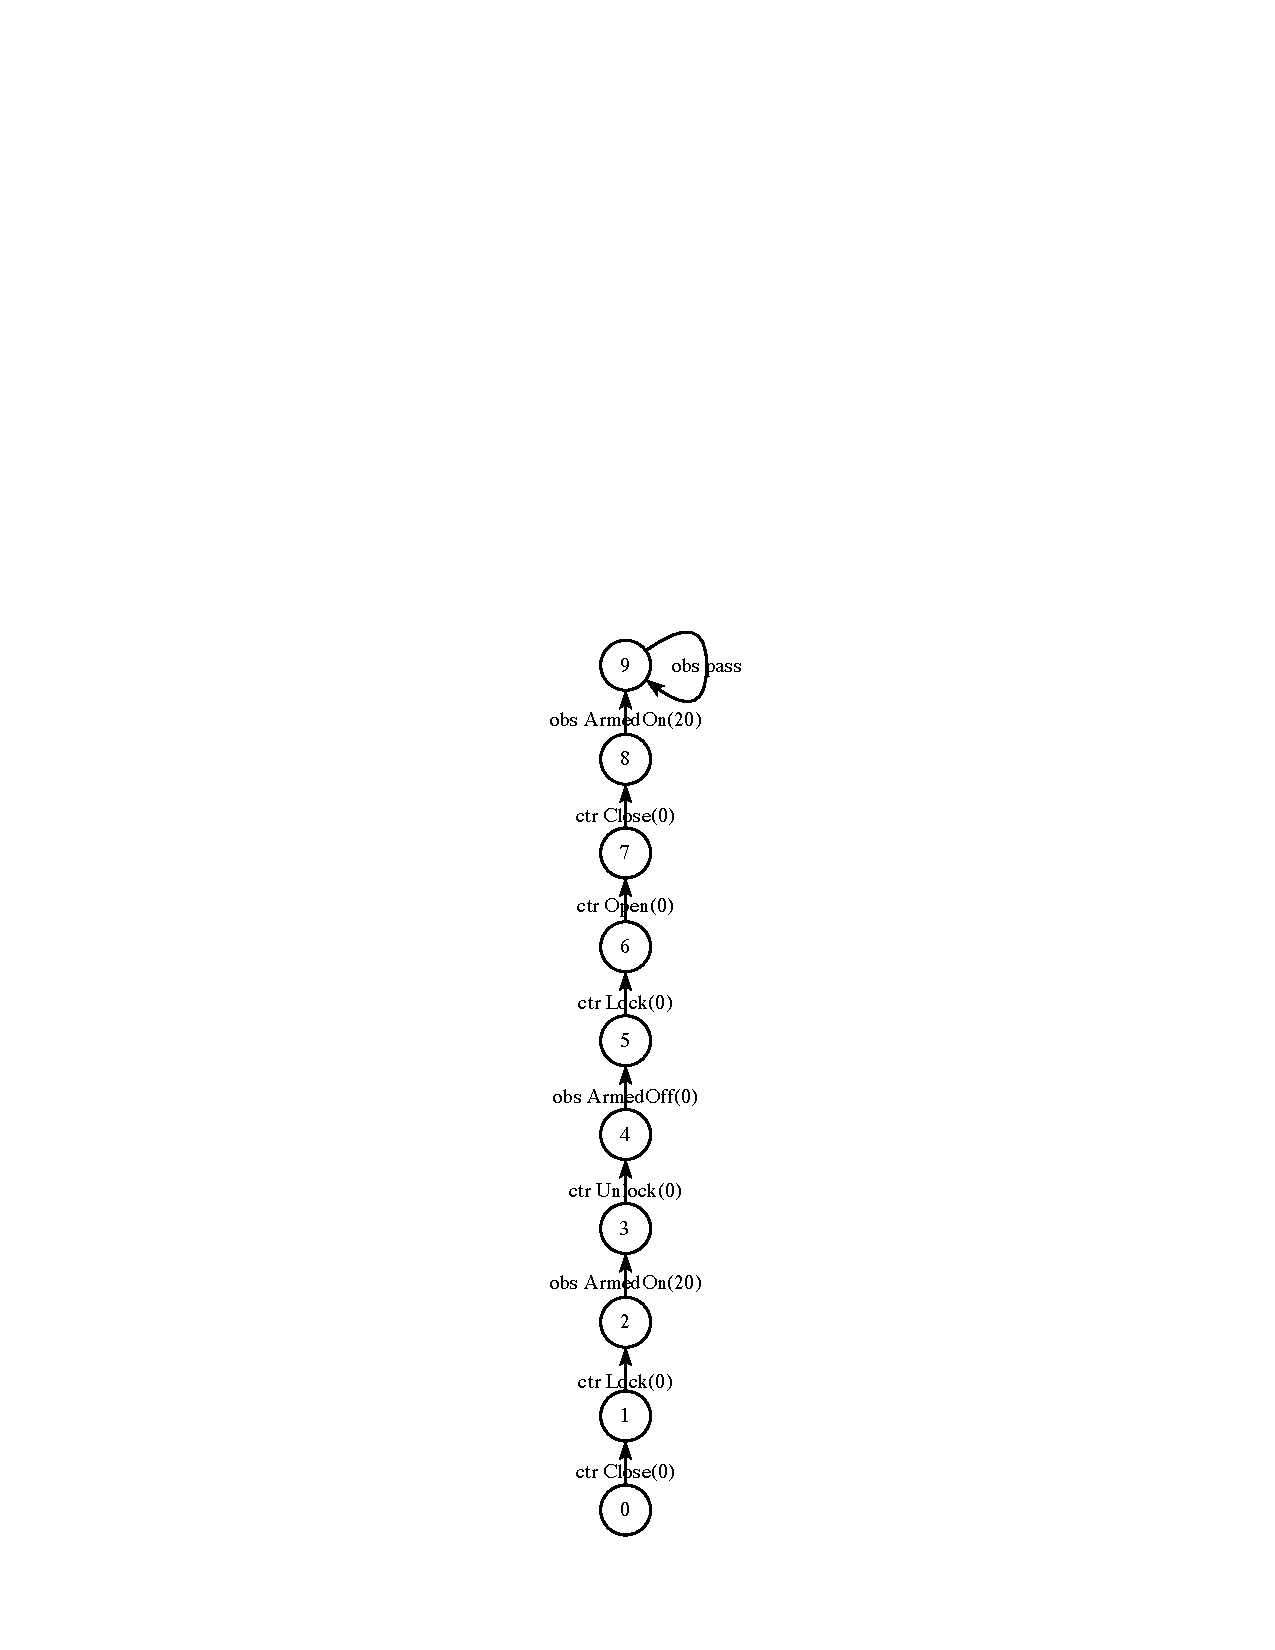
\includegraphics{figures/cas1_tc1}
}
\end{minipage}
\hspace{0.04\textwidth}
\begin{minipage}[T]{0.15\textwidth}
  \resizebox{!}{0.7\textheight}{
  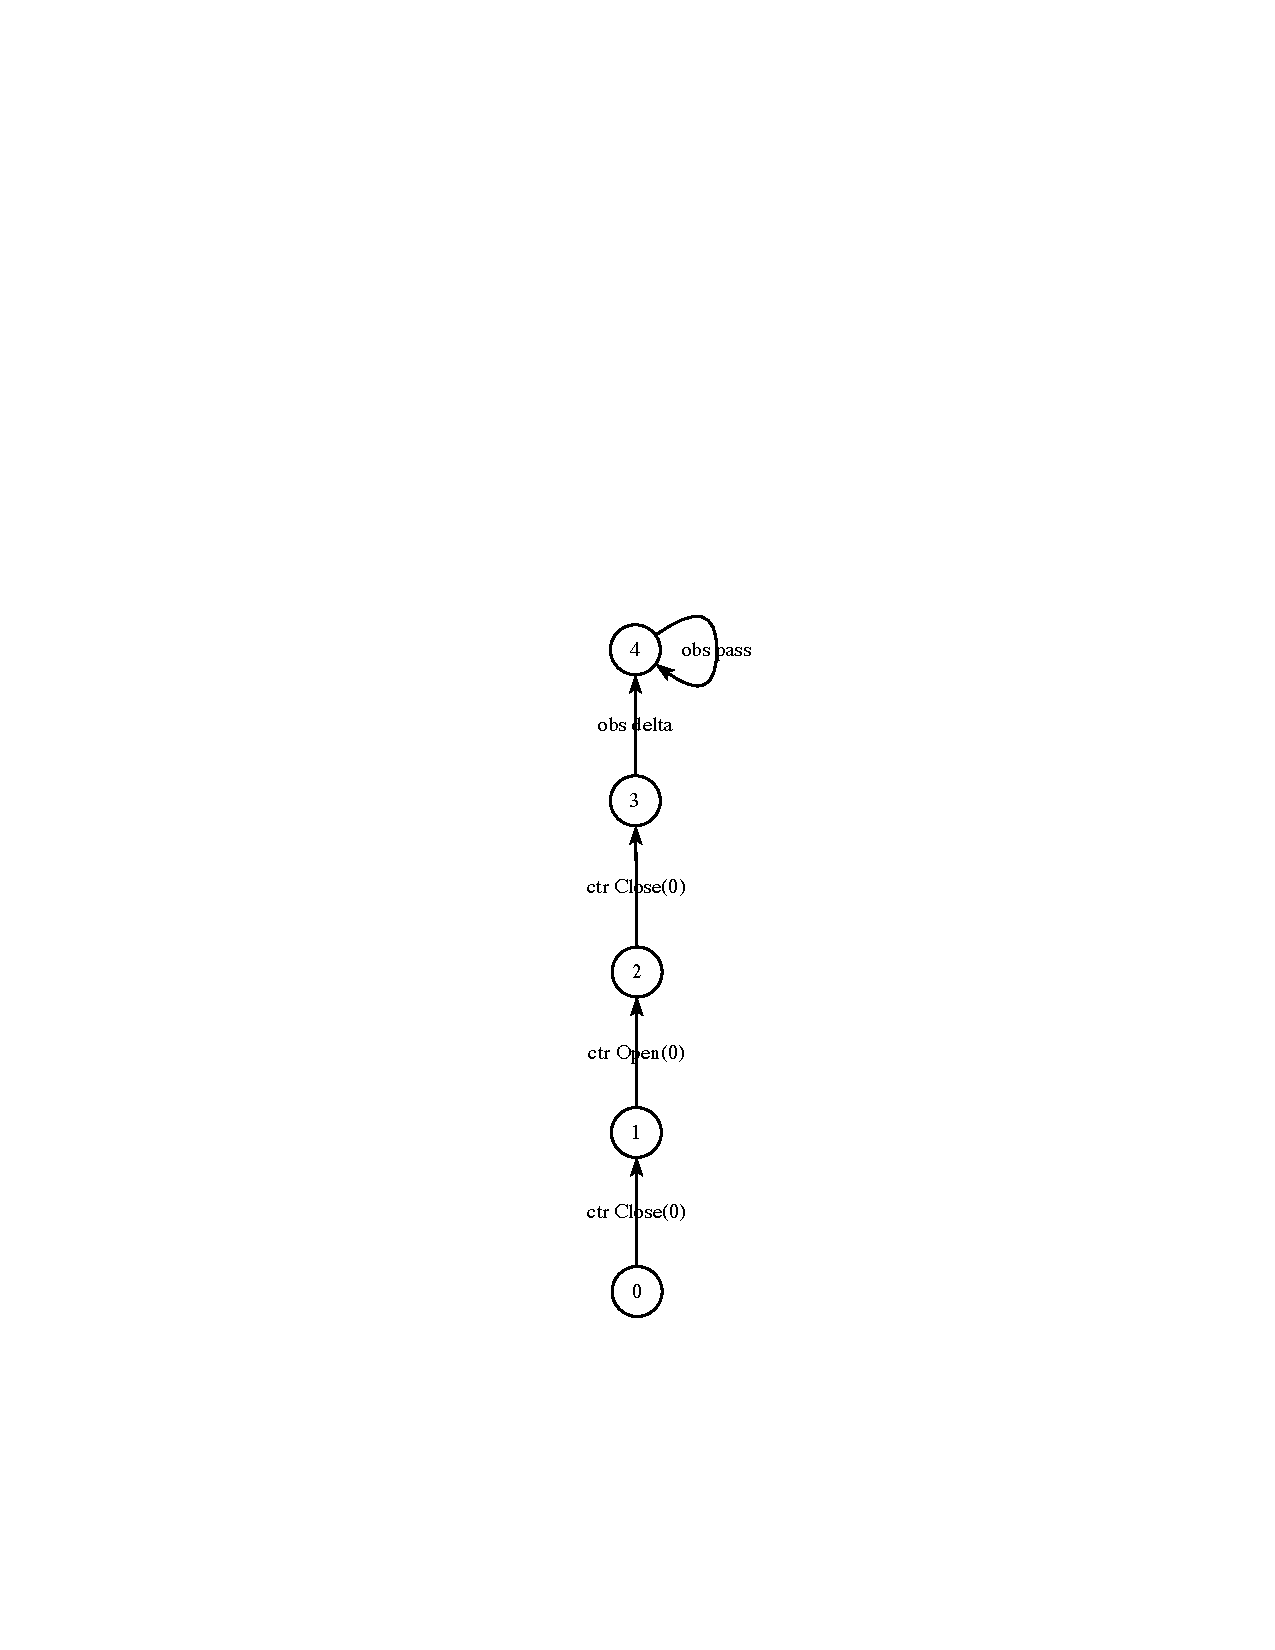
\includegraphics{figures/cas1_tc4}
}
\end{minipage}
\hspace{0.04\textwidth}
\begin{minipage}[T]{0.15\textwidth}
  \resizebox{!}{0.7\textheight}{
  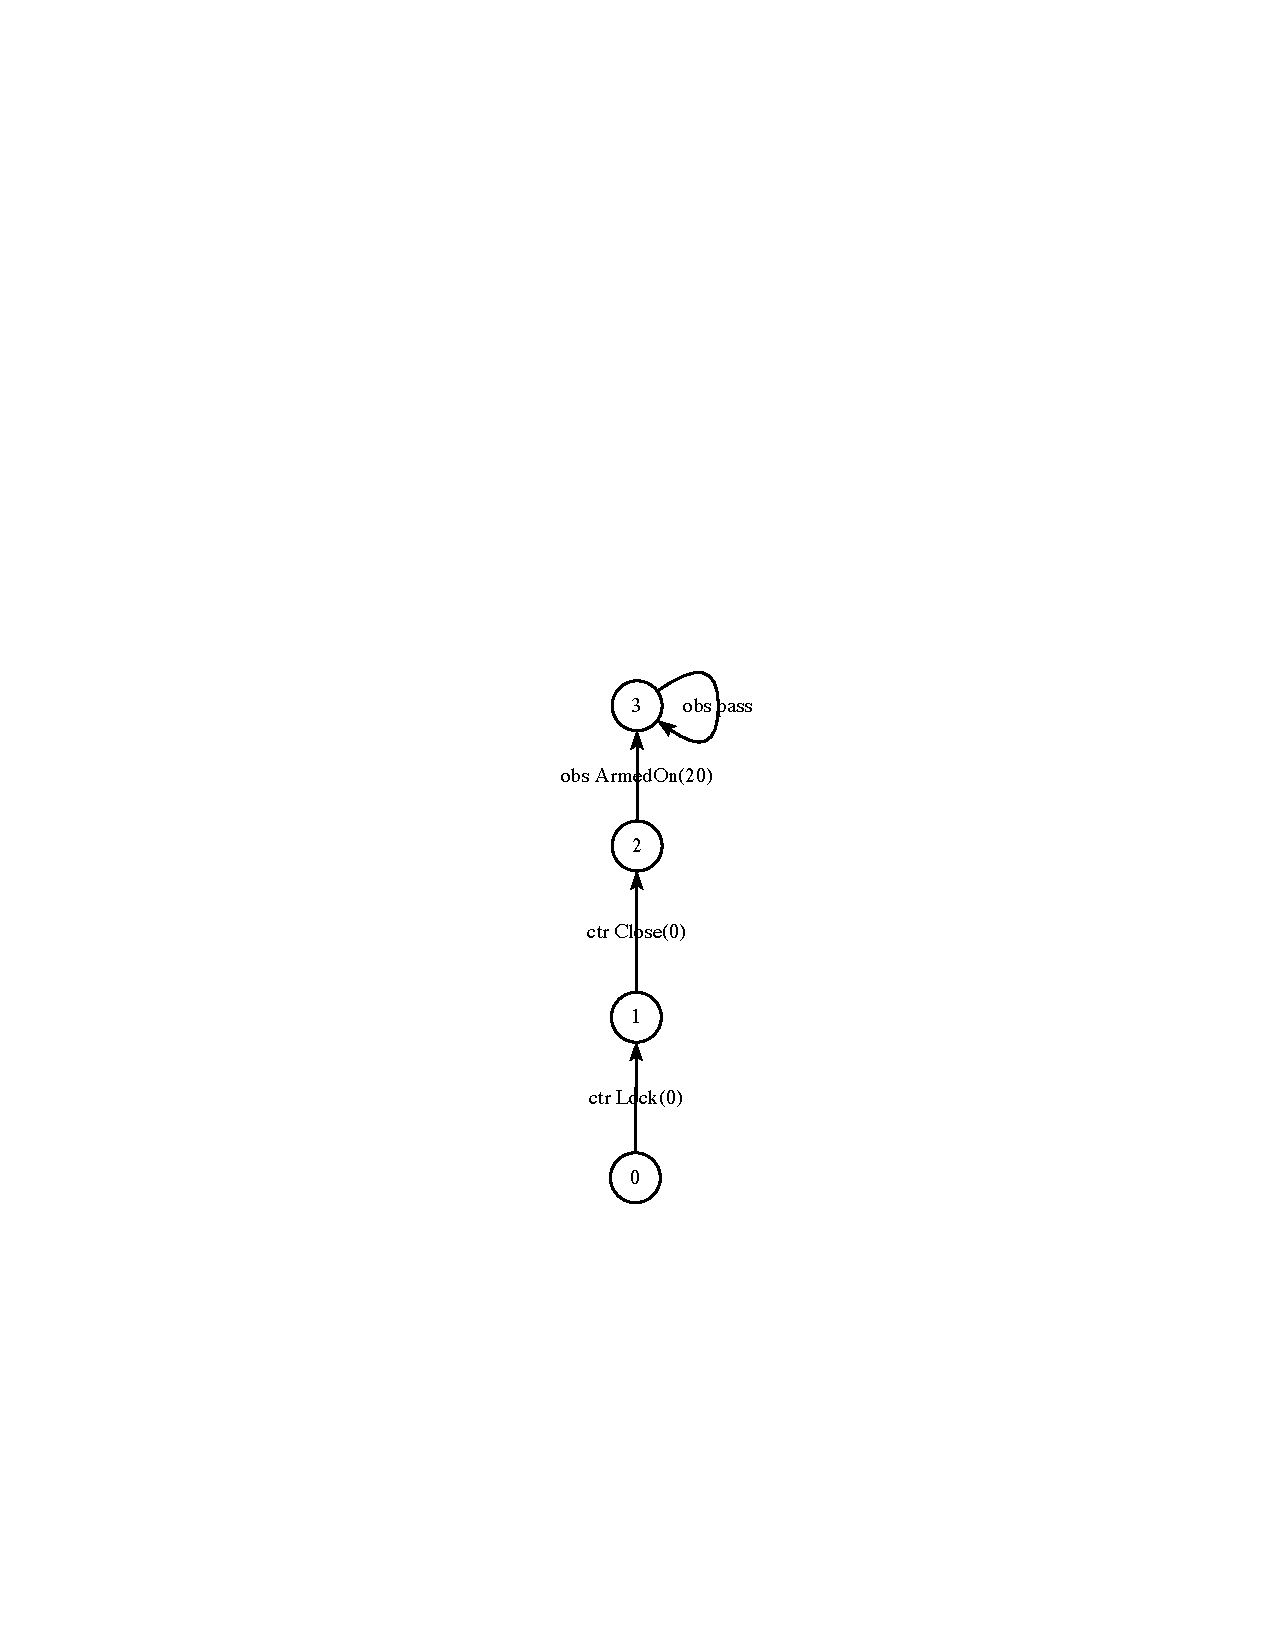
\includegraphics{figures/cas1_tc2}
}
\end{minipage}
\hspace{0.04\textwidth}
\begin{minipage}[T]{0.4\textwidth}
  \resizebox{!}{0.7\textheight}{
  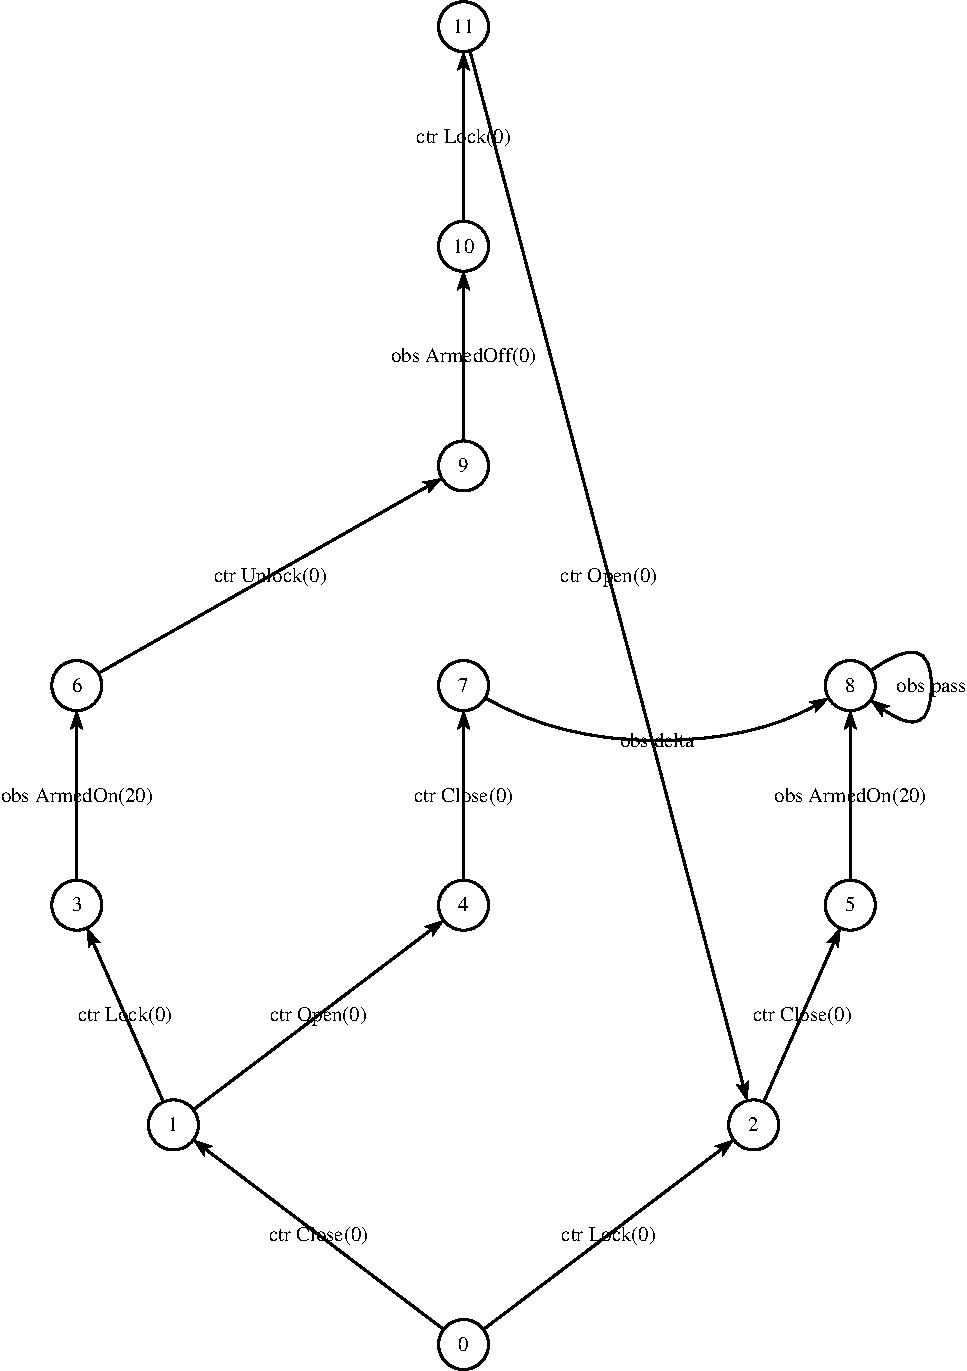
\includegraphics[height=.7\textheight]{figures/3merged_trace_cropped}
}
\end{minipage}

\end{frame}

\subsection{Verify Test Cases}
\begin{frame}
  \frametitle{Verify Test Cases}
  \begin{itemize}
    \item Two kinds of properties
    \begin{itemize}
      \item Safety properties
      \item Completeness properties (inclusion of specific scenarios)
    \end{itemize}
    \item CADP Evaluator tool
    \item regular alternation-free mu-calculus formula
  \end{itemize}
\end{frame}

\begin{frame}
  \frametitle{Verify Test Cases cont.}
Sample safety property
\begin{alltt}\footnotesize

[({\bfseries not} '{\color{blue}ctr Lock.*}')* .

'{\color{blue}ctr Close.*}' .

({\bfseries not} '{\color{blue}ctr Open.*}')*  . '{\color{blue}ctr Lock.*}' .

({\bfseries not} ('{\color{blue}obs ArmedOn(20)}' or '{\color{blue}ctr .*(.)}' {\bfseries or}

'{\color{blue}ctr .*(1.)}' {\bfseries or} '{\color{blue}obs pass}'))] {\bfseries false}
\end{alltt}

{\color{green} \Huge \raggedright \cmark}
\end{frame}

\begin{frame}
  \frametitle{Verify Test Cases cont.}
Inclusion of Scenario
\begin{alltt}\footnotesize
(<{\bfseries true}*> <'{\color{blue}obs SoundOff.*}'>
<'{\color{blue}obs FlashOff.*}'> {\bfseries true})

{\bfseries or}

(<{\bfseries true}*> <'{\color{blue}obs FlashOff.*}'>
<'{\color{blue}obs SoundOff.*}'> {\bfseries true})
\end{alltt}  
{\color{red} \Huge \raggedright \xmark}
\end{frame}

\subsection{Results - Iteration 1}
\begin{frame}
  \frametitle{Results}
  \vspace{-1.2cm}
\begin{table}
\begin{tiny}
\caption{Quality check of the test cases over the iterations,
    measured in mutation score on the faulty implementations and by model checking of the merged test cases.}\end{tiny}
\centering
\resizebox{0.99\textwidth}{!}{
 \begin{tabular}{l|c|c|c|c|c|c}
   & \# Mutants & \# Test cases & Mutation Score & Safety & Completeness & Purposes \\
\hline \onslide
$\mbox{CAS}_1$ & 114 & 12 & 81\% &\cellcolor<2>{yellow} 18/18 & \cellcolor<2>{white}\cellcolor<3>{yellow}10/25 & \cellcolor<3>{white} 3/8\\
%$\mbox{CAS}_2$ & 1889 & 17 & 73\% & 18/18 & 24/25 & 8/8 \onslide<4->\\
%$\mbox{CAS}_{1+2}$ & 2003 & 29 & 97\% & 18/18 & 25/25 & 8/8 \onslide<5->\\
%$\mbox{CAS}_3$ & 2179 & 53 & 100\% & 18/18 & 25/25 & 8/8 \onslide<6->\\
%$\mbox{CAS}_{1+2+3}$& 2179 & 54 & 100\% & 18/18 & 25/25 & 8/8 \onslide<7->\\
\end{tabular}}
%\vspace{0.9cm}
\label{tab:cas_tcg}
\end{table}
\begin{itemize}
  \item \onslide<2-> All safety properties fulfilled
  \item \onslide<2-> Violation would imply test model is incorrect
  \item \onslide<3> Not complete
\end{itemize}

\end{frame}

%\begin{frame}
%  \frametitle{Implementation and Refactoring}
%\end{frame}


%%%%%%%%%%%%%%%%%%%%%%%%%%%%%%%%%%%%%%%%%%%%%%%%%%%%%%%%%%%%%%%%%%%%%%%%%%%%
%\section{Empirical Results}
%%%%%%%%%%%%%%%%%%%%%%%%%%%%%%%%%%%%%%%%%%%%%%%%%%%%%%%%%%%%%%%%%%%%%%%%%%%%

\section{Iteration 2}
\subsection{Model}
%\subsection{Partial Models}
\begin{frame}
  \frametitle{Partial Models}
\vspace{-0.2cm}
\begin{minipage}[T]{0.29\textwidth}
\centering
  \resizebox{!}{0.65\textheight}{
    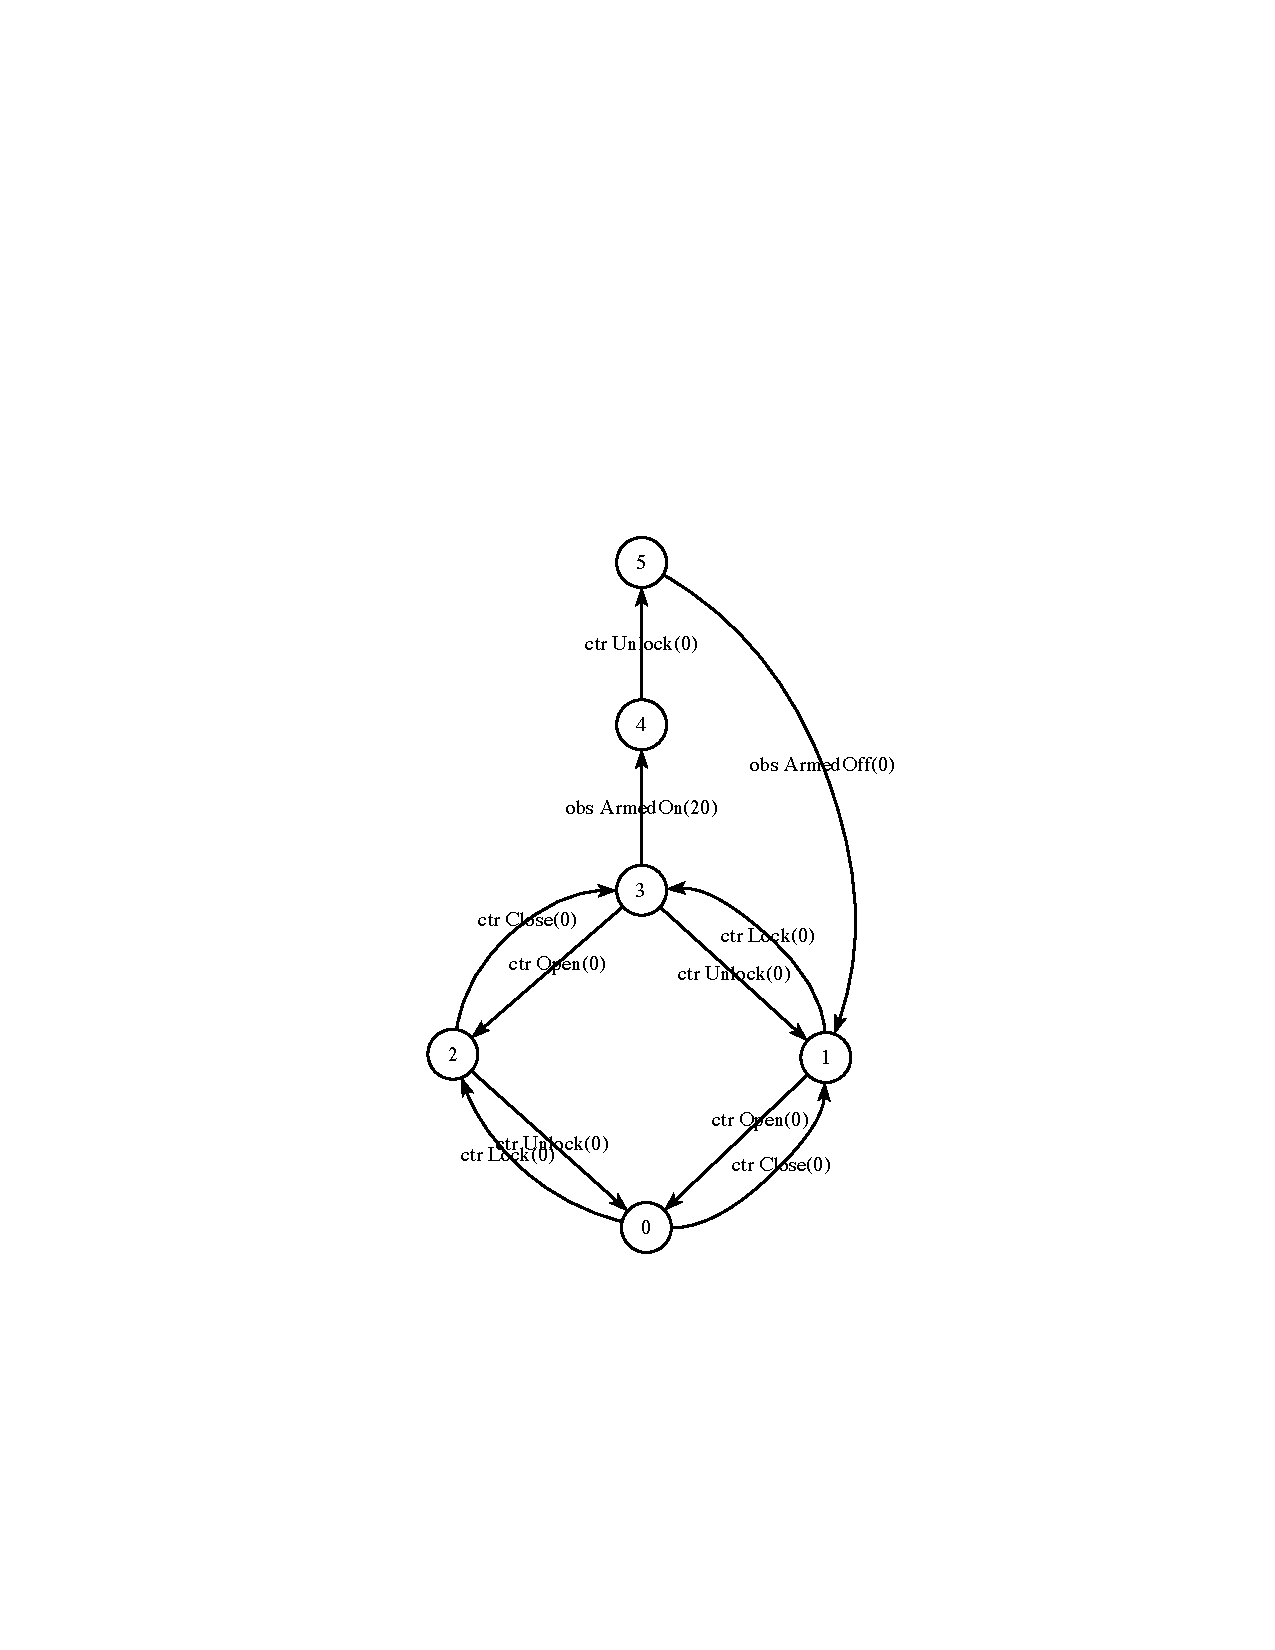
\includegraphics{figures/cas1}
}
$CAS_1$
\end{minipage}
\hspace{0.04\textwidth}
\begin{minipage}[T]{0.29\textwidth}
\centering
  \resizebox{!}{0.65\textheight}{
    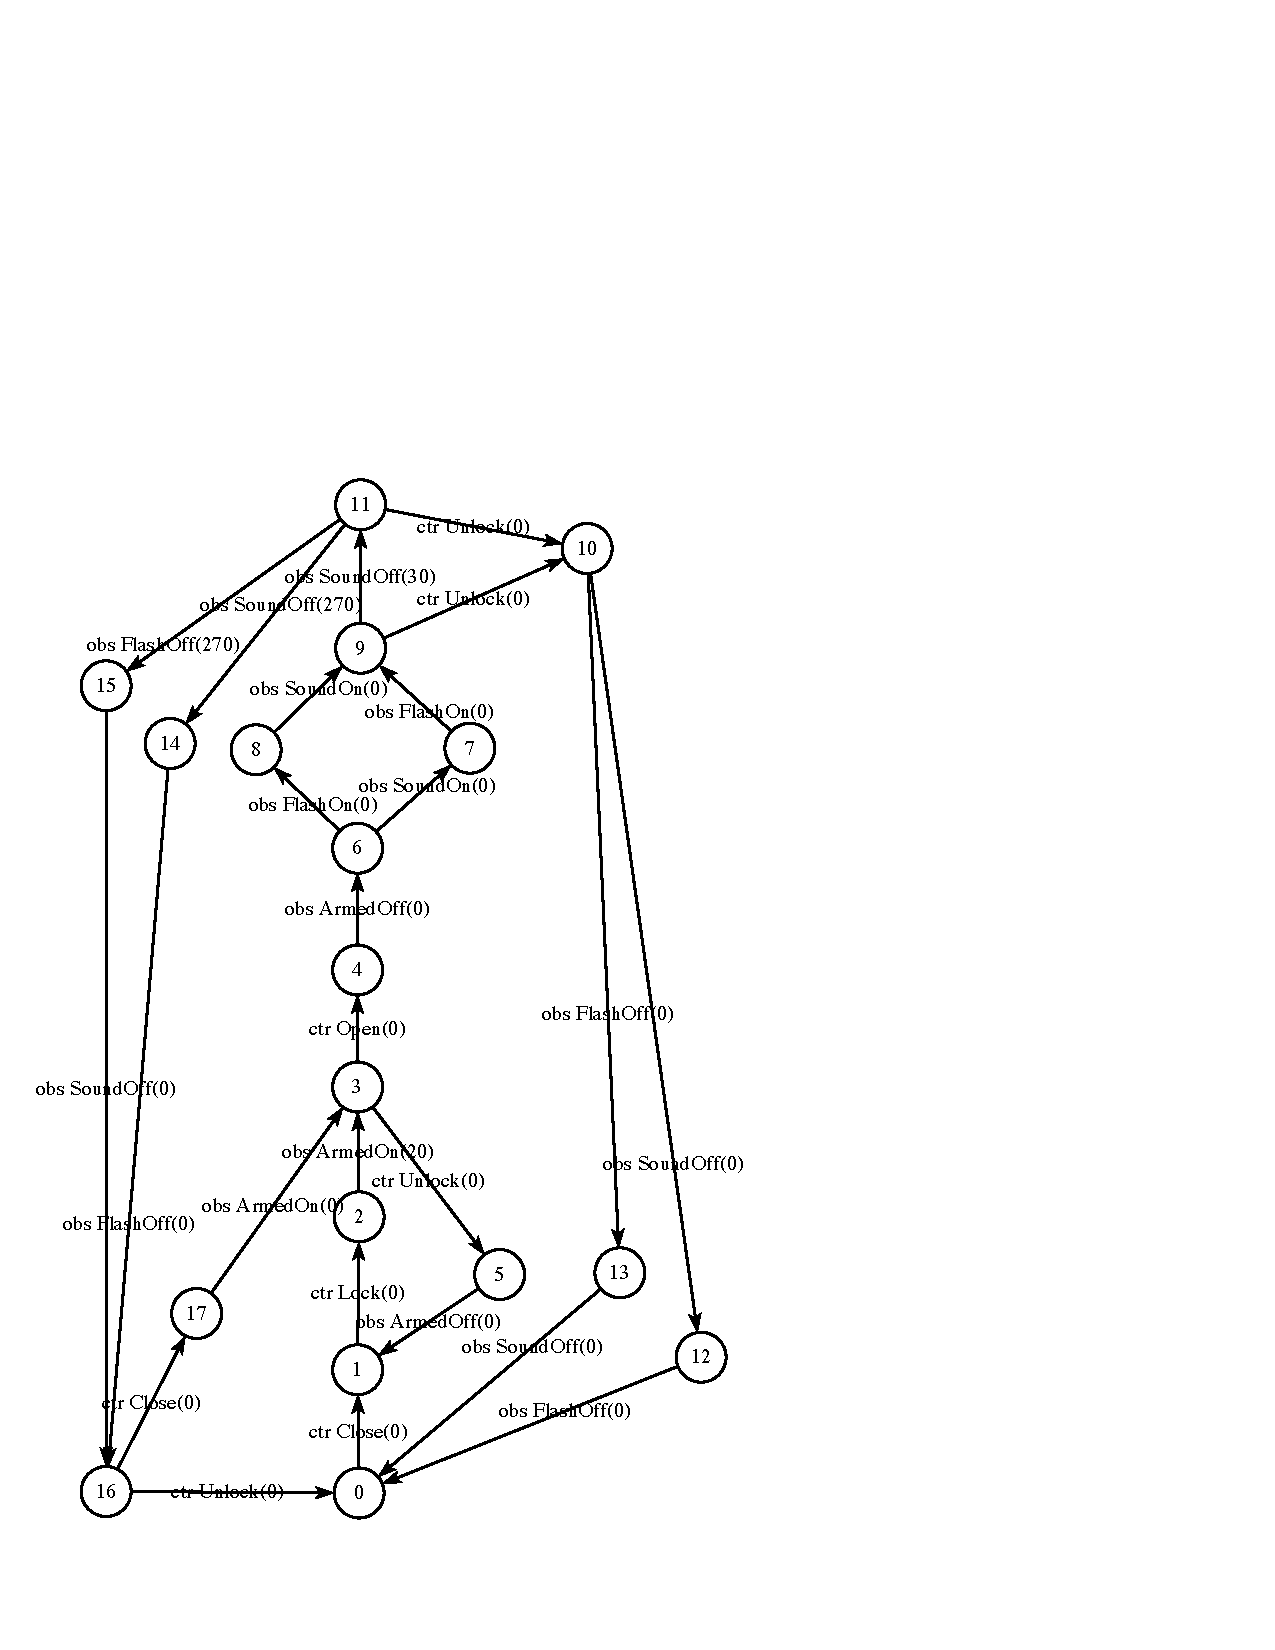
\includegraphics{figures/cas2}
}
$CAS_2$
\end{minipage}
%\hspace{0.04\textwidth}
%\begin{minipage}[T]{0.29\textwidth}
%\centering
%  \resizebox{!}{0.6\textheight}{
%    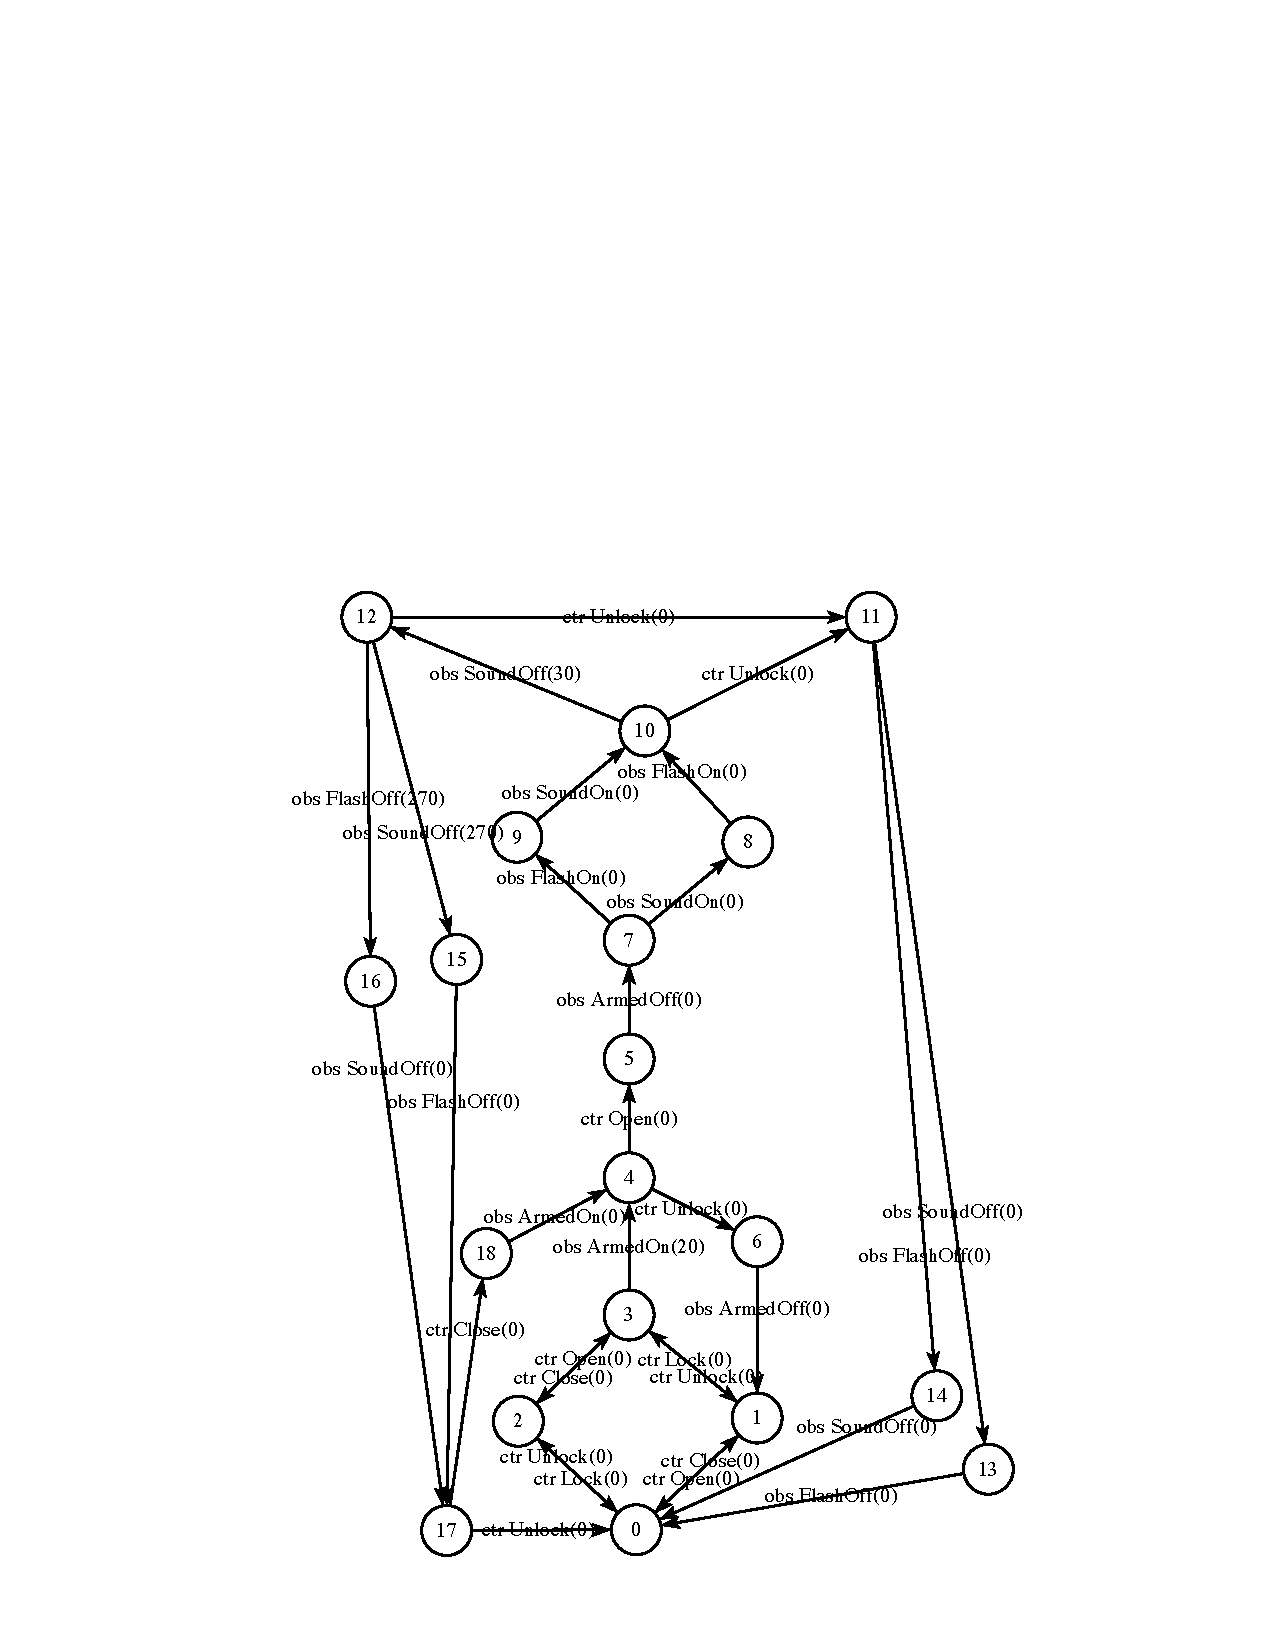
\includegraphics{figures/cas3}
%}
%$CAS_3$
%\end{minipage}
\end{frame}
\subsection{Results}
\begin{frame}
  \frametitle{Results - Iteration 2}
  \vspace{-1.2cm}
\begin{table}
\begin{tiny}
\caption{Quality check of the test cases over the iterations,
    measured in mutation score on the faulty implementations and by model checking of the merged test cases.}\end{tiny}
\centering
\resizebox{0.99\textwidth}{!}{
 \begin{tabular}{l|c|c|c|c|c|c}
   & \# Mutants & \# Test cases & Mutation Score & Safety & Completeness & Purposes \\
\hline \onslide
$\mbox{CAS}_1$ & 114 & 12 & 81\% & 18/18 & 10/25 & 3/8\onslide\\
$\mbox{CAS}_2$ & 1889 & 17 & 73\% & 18/18 & 24/25 & 8/8 \onslide<2->\\
$\mbox{CAS}_{1+2}$ & 2003 & 29 & \cellcolor<4>{yellow} 97\% & \cellcolor<4>{white} 18/18 & \cellcolor<3>{yellow} 25/25 & \cellcolor<3>{white} 8/8\onslide\\
%$\mbox{CAS}_3$ & 2179 & 53 & 100\% & 18/18 & 25/25 & 8/8 \onslide<6->\\
%$\mbox{CAS}_{1+2+3}$& 2179 & 54 & 100\% & 18/18 & 25/25 & 8/8 \onslide<7->\\
\end{tabular}}
%\vspace{0.9cm}
%\onslide<3->
\label{tab:cas_tcg}
\end{table}
\onslide<3->
\begin{itemize}
  \item \onslide<3-> Together complete in respect to properties
  \item \onslide<4> One faulty implementation still not detected 
\end{itemize}

\end{frame}


\section{Iteration 3}
\subsection{Model}
\vspace{-0.2cm}
%\subsection{Partial Models}
\begin{frame}
  \frametitle{Partial Models}
\begin{minipage}[T]{0.29\textwidth}
\centering
  \resizebox{!}{0.65\textheight}{
    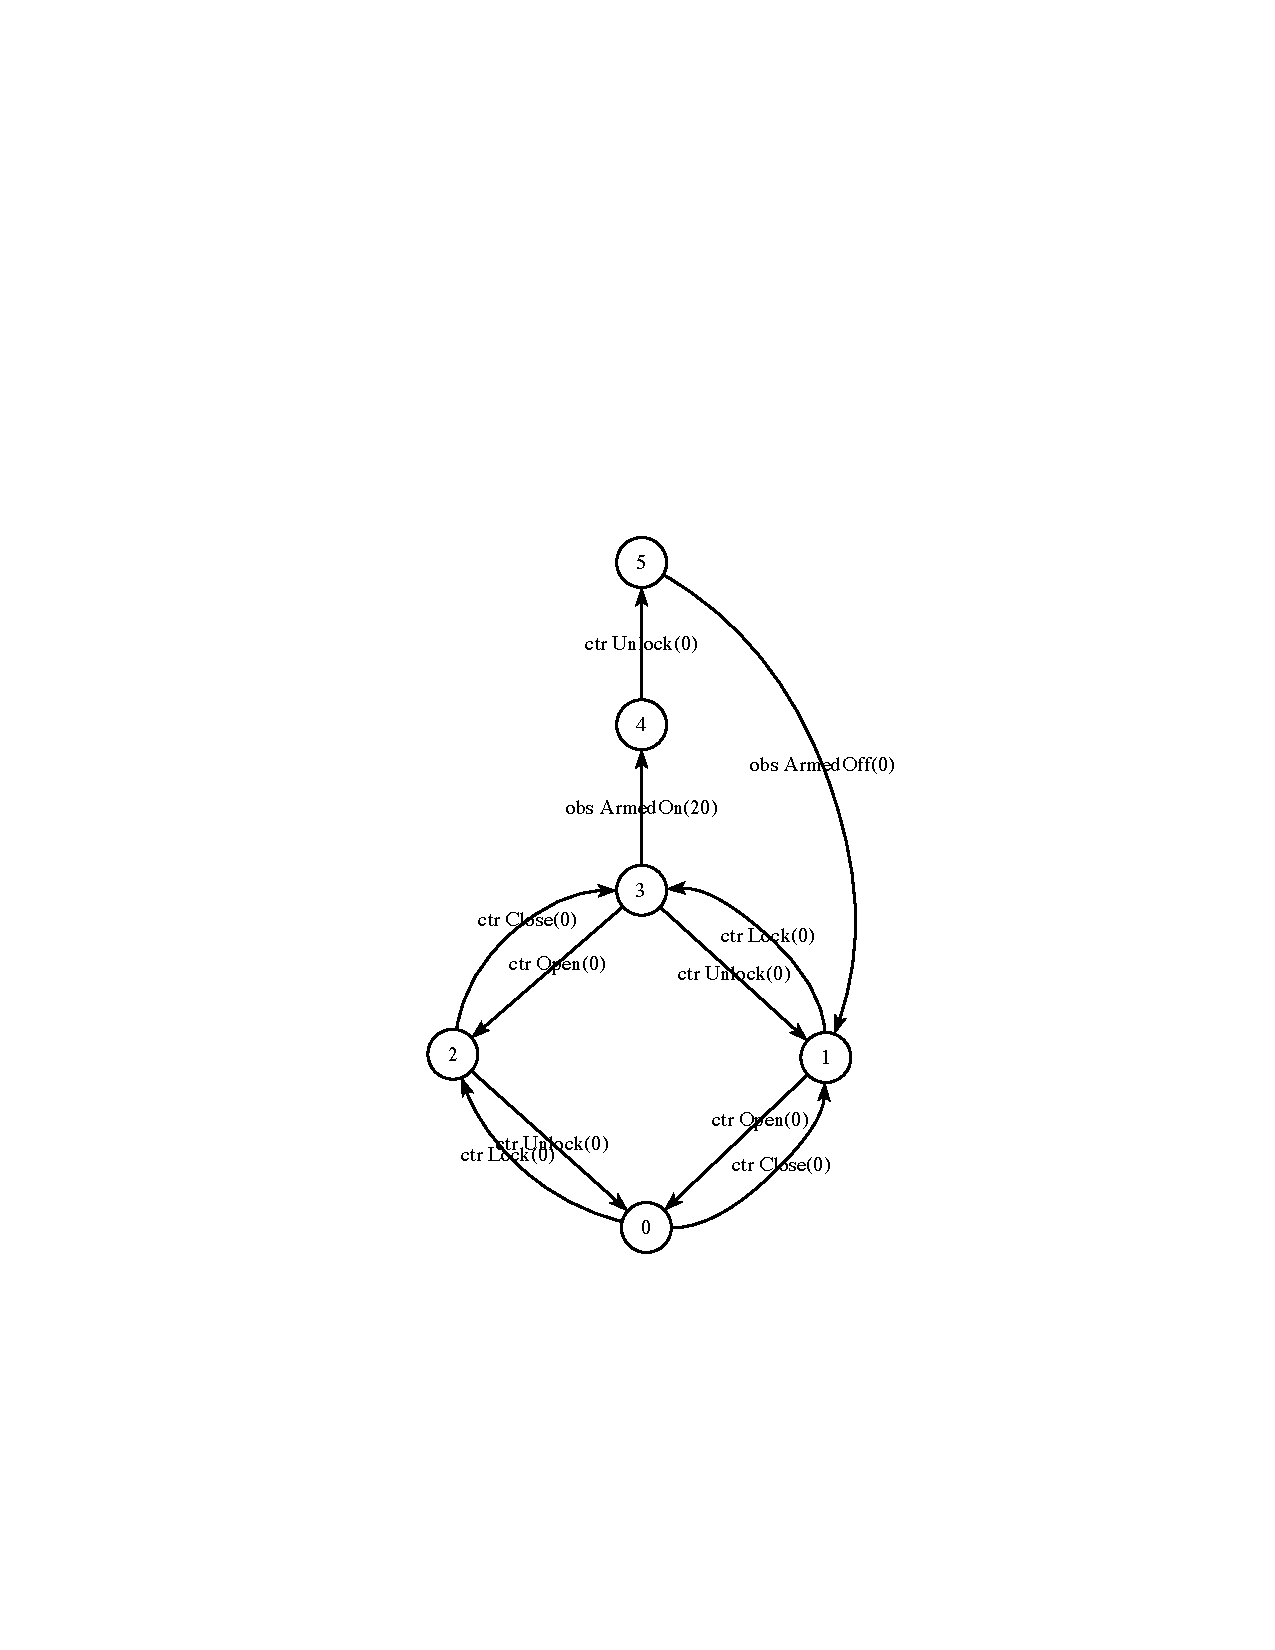
\includegraphics{figures/cas1}
}
$CAS_1$
\end{minipage}
\hspace{0.04\textwidth}
\begin{minipage}[T]{0.29\textwidth}
\centering
  \resizebox{!}{0.65\textheight}{
    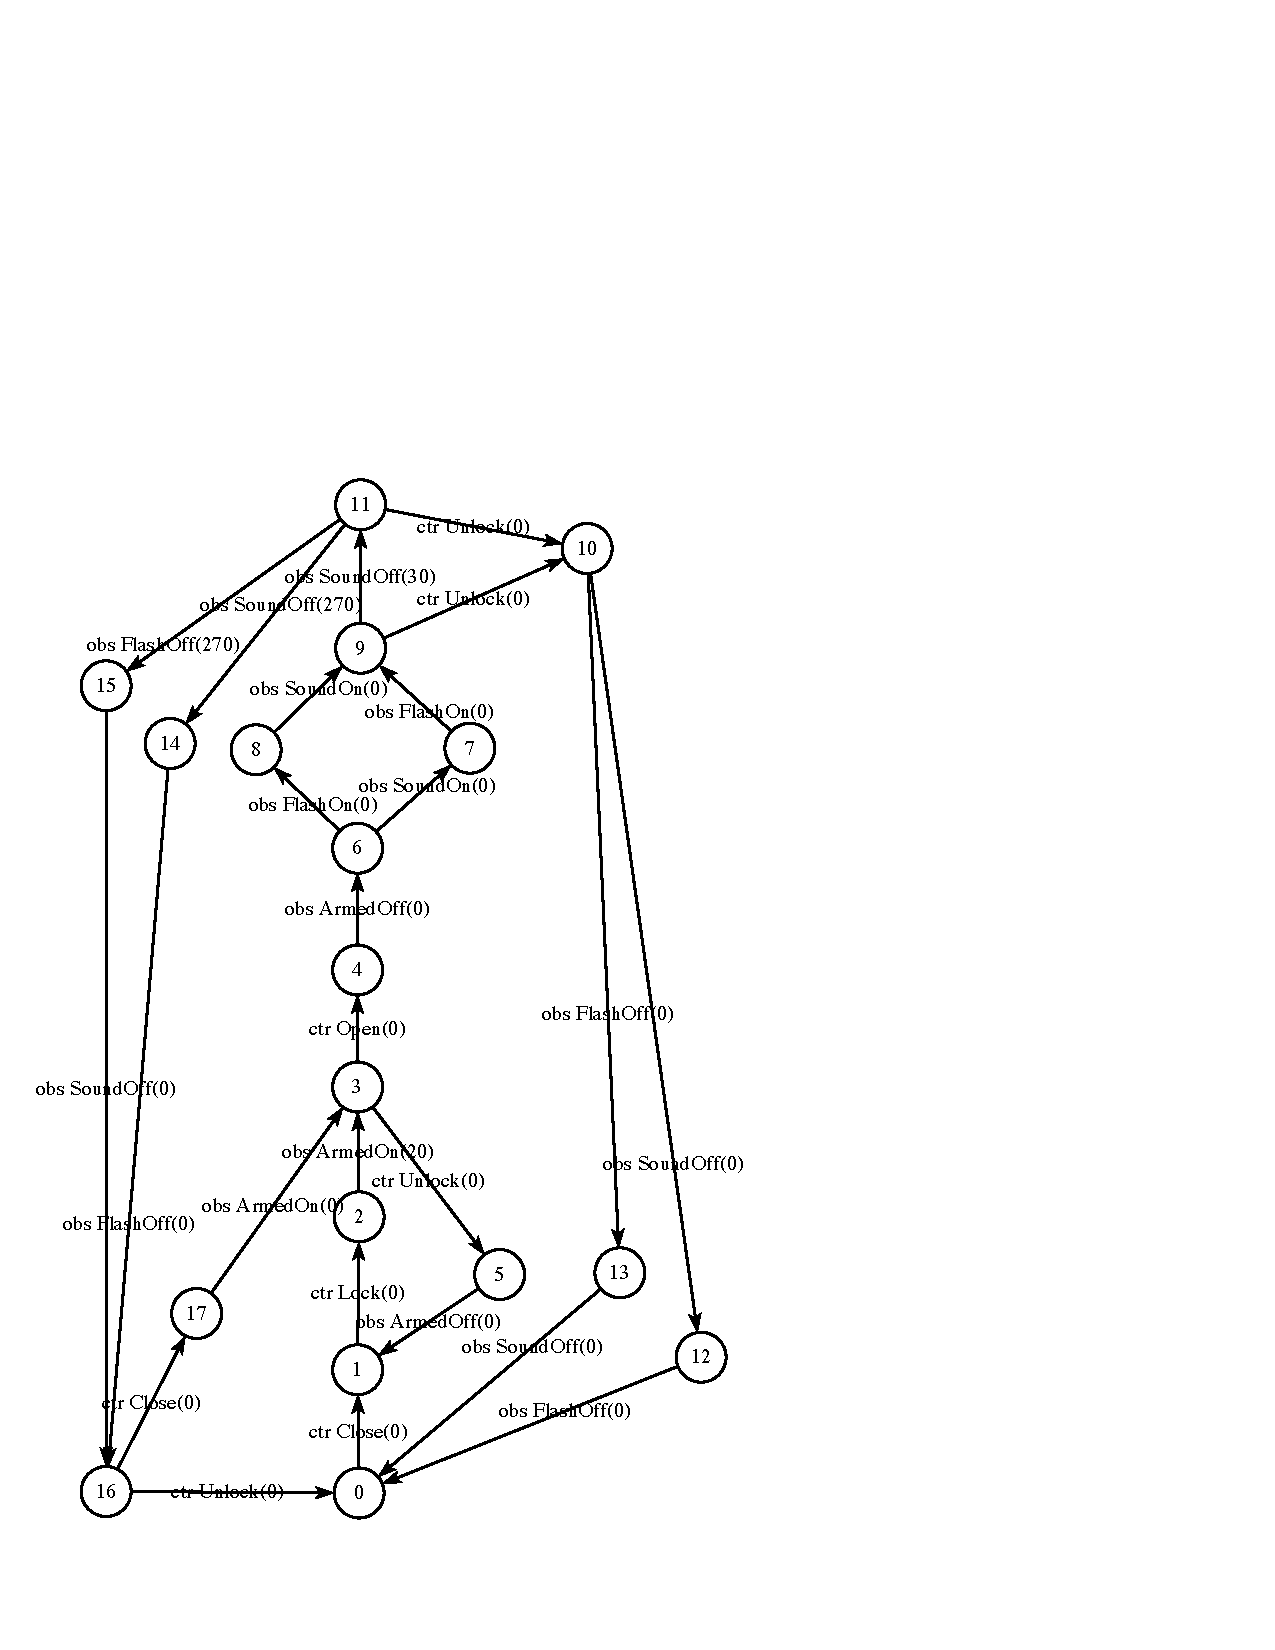
\includegraphics{figures/cas2}
}
$CAS_2$
\end{minipage}
\hspace{0.04\textwidth}
\begin{minipage}[T]{0.29\textwidth}
\centering
  \resizebox{!}{0.65\textheight}{
    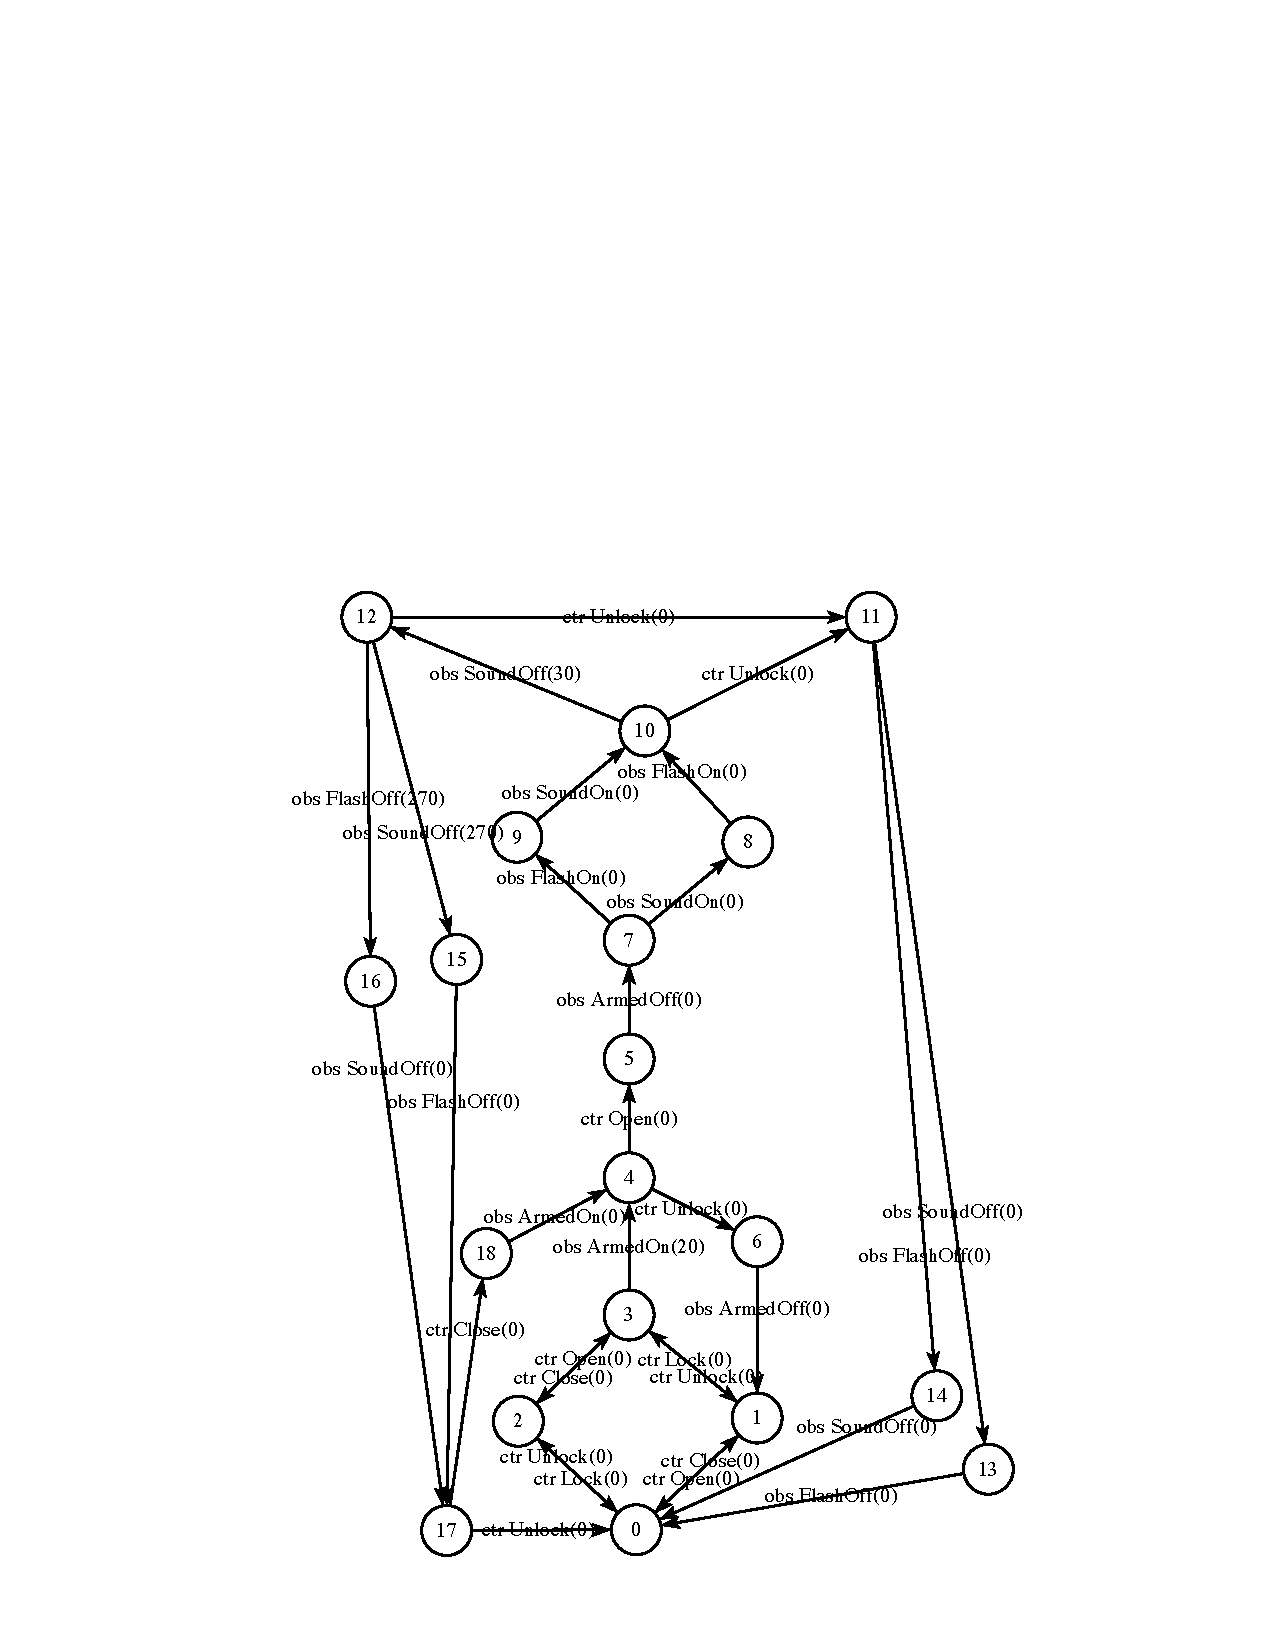
\includegraphics{figures/cas3}
}
$CAS_3$
\end{minipage}
\end{frame}
\subsection{Results}

\begin{frame}
  \frametitle{Results - Iteration 3}
  \vspace{-1.2cm}
\begin{table}
\begin{tiny}
\caption{Quality check of the test cases over the iterations,
    measured in mutation score on the faulty implementations and by model checking of the merged test cases.}\end{tiny}
\centering
\resizebox{0.99\textwidth}{!}{
 \begin{tabular}{l|c|c|c|c|c|c}
   & \# Mutants & \# Test cases & Mutation Score & Safety & Completeness & Purposes \\
\hline \onslide
$\mbox{CAS}_1$ & 114 & 12 & 81\% & 18/18 & 10/25 & 3/8\\
$\mbox{CAS}_2$ & 1889 & 17 & 73\% & 18/18 & 24/25 & 8/8\\
$\mbox{CAS}_{1+2}$ & 2003 & 29 & 97\% & 18/18 & 25/25 & 8/8\\
$\mbox{CAS}_3$ & 2179 & 53 & \cellcolor<2>{yellow}100\% & \cellcolor<2>{white} 18/18 & 25/25 & 8/8\\
%$\mbox{CAS}_{1+2+3}$& 2179 & 54 & 100\% & 18/18 & 25/25 & 8/8 \onslide\\
\end{tabular}}

\label{tab:cas_tcg}
\end{table}
\begin{itemize}
  \onslide<2> \item All faulty implementations detected
\end{itemize}
\end{frame}

\begin{frame}
  \frametitle{Results - Iteration 3 (incremental)}
  \vspace{-1.2cm}
\begin{table}
\begin{tiny}
\caption{Quality check of the test cases over the iterations,
    measured in mutation score on the faulty implementations and by model checking of the merged test cases.}\end{tiny}
\centering
\resizebox{0.99\textwidth}{!}{
 \begin{tabular}{l|c|c|c|c|c|c}
   & \# Mutants & \# Test cases & Mutation Score & Safety & Completeness & Purposes \\
\hline \onslide
$\mbox{CAS}_1$ & 114 & 12 & 81\% & 18/18 & 10/25 & 3/8\\
$\mbox{CAS}_2$ & 1889 & 17 & 73\% & 18/18 & 24/25 & 8/8\\
$\mbox{CAS}_{1+2}$ & 2003 & 29 & 97\% & 18/18 & 25/25 & 8/8\\
$\mbox{CAS}_3$ & 2179 & \cellcolor<2>{yellow}53 & \cellcolor<2>{white}100\% & 18/18 & 25/25 & 8/8\\
$\mbox{CAS}_{1+2+3}$& 2179 & \cellcolor<2>{yellow}54 & \cellcolor<2>{white} 100\% & 18/18 & 25/25 & 8/8\\
\end{tabular}}
\vspace{0.9cm}
\begin{itemize}
  \item Reuse existing test cases
  \onslide<2> \item Size of test suite only increases slightly
\end{itemize}

\label{tab:cas_tcg}
\end{table}
\end{frame}



%%%%%%%%%%%%%%%%%%%%%%%%%%%%%%%%%%%%%%%%%%%%%%%%%%%%%%%%%%%%%%%%%%%%%%%%%%%%
\section{Discussion}
%%%%%%%%%%%%%%%%%%%%%%%%%%%%%%%%%%%%%%%%%%%%%%%%%%%%%%%%%%%%%%%%%%%%%%%%%%%%

\subsection{Benefits}
\begin{frame}
  \frametitle{Discussion - Benefits}
Benefits
    \begin{itemize}
      \item Advantages of three disciplines
      \begin{enumerate}
        \item Model-based testing\\
          $\rightarrow$ generate test cases automatically and systematically
        \item Test-driven development\\
          $\rightarrow$ put test cases into center of development
        \item Formal methods\\
          $\rightarrow$ check test cases against requirements (traceability!)
      \end{enumerate}
    \end{itemize}
\end{frame}

\subsection{Limitations}
\begin{frame}
  \frametitle{Discussion - Limitations}
Limitations
    \begin{itemize}
      \item Model checking test cases
      \begin{itemize}
        \item Many test cases required for model-checking
        \item Future work: model learning
      \end{itemize}
      \item Mutation approach
      \begin{itemize}
        \item Many generated model mutants -- 22 CPU hours for $CAS_3$
        \item Future work: mutation avoidance
      \end{itemize}
    \end{itemize}
\end{frame}



% \begin{frame}
%   \frametitle{Discussion - Benefits and Limitations}
%   \begin{itemize}
%     \item{Benefits}
%       \begin{itemize}
%         \item No need to update test cases
%         \item System changes $\rightarrow$ update test model
%         \item Interface changes $\rightarrow$ update test adapter
%         \item Test models can be checked for certain properties
%         \item Vertical (refinement) steps can be checked
%       \end{itemize}
%     \item{Limitations}
%       \begin{itemize}
%         \item Test adapter has to be written additionally
%       \end{itemize}
%   \end{itemize}
% \end{frame}







%%%%%%%%%%%%%%%%%%%%%%%%%%%%%%%%%%%%%%%%%%%%%%%%%%%%%%%%%%%%%%%%%%%%%%%%%%%%
\section{Conclusion}
%%%%%%%%%%%%%%%%%%%%%%%%%%%%%%%%%%%%%%%%%%%%%%%%%%%%%%%%%%%%%%%%%%%%%%%%%%%%
\begin{frame}
  \frametitle{Conclusion}
\vspace{-0.2cm}
\begin{minipage}[T]{0.55\textwidth}
  \begin{itemize}
    \item Combination of
    \begin{enumerate}
      \item Model-based testing
      \item Test-driven development
      \item Formal methods
    \end{enumerate}
    \item Model refinement
    \begin{itemize}
      \item Partial test models
      \item Underspecification
    \end{itemize}
    \item Verification of Test Cases
  \end{itemize}
\end{minipage}
\hspace{0.04\textwidth}
\begin{minipage}[T]{0.35\textwidth}
  \resizebox{!}{0.5\textheight}{
  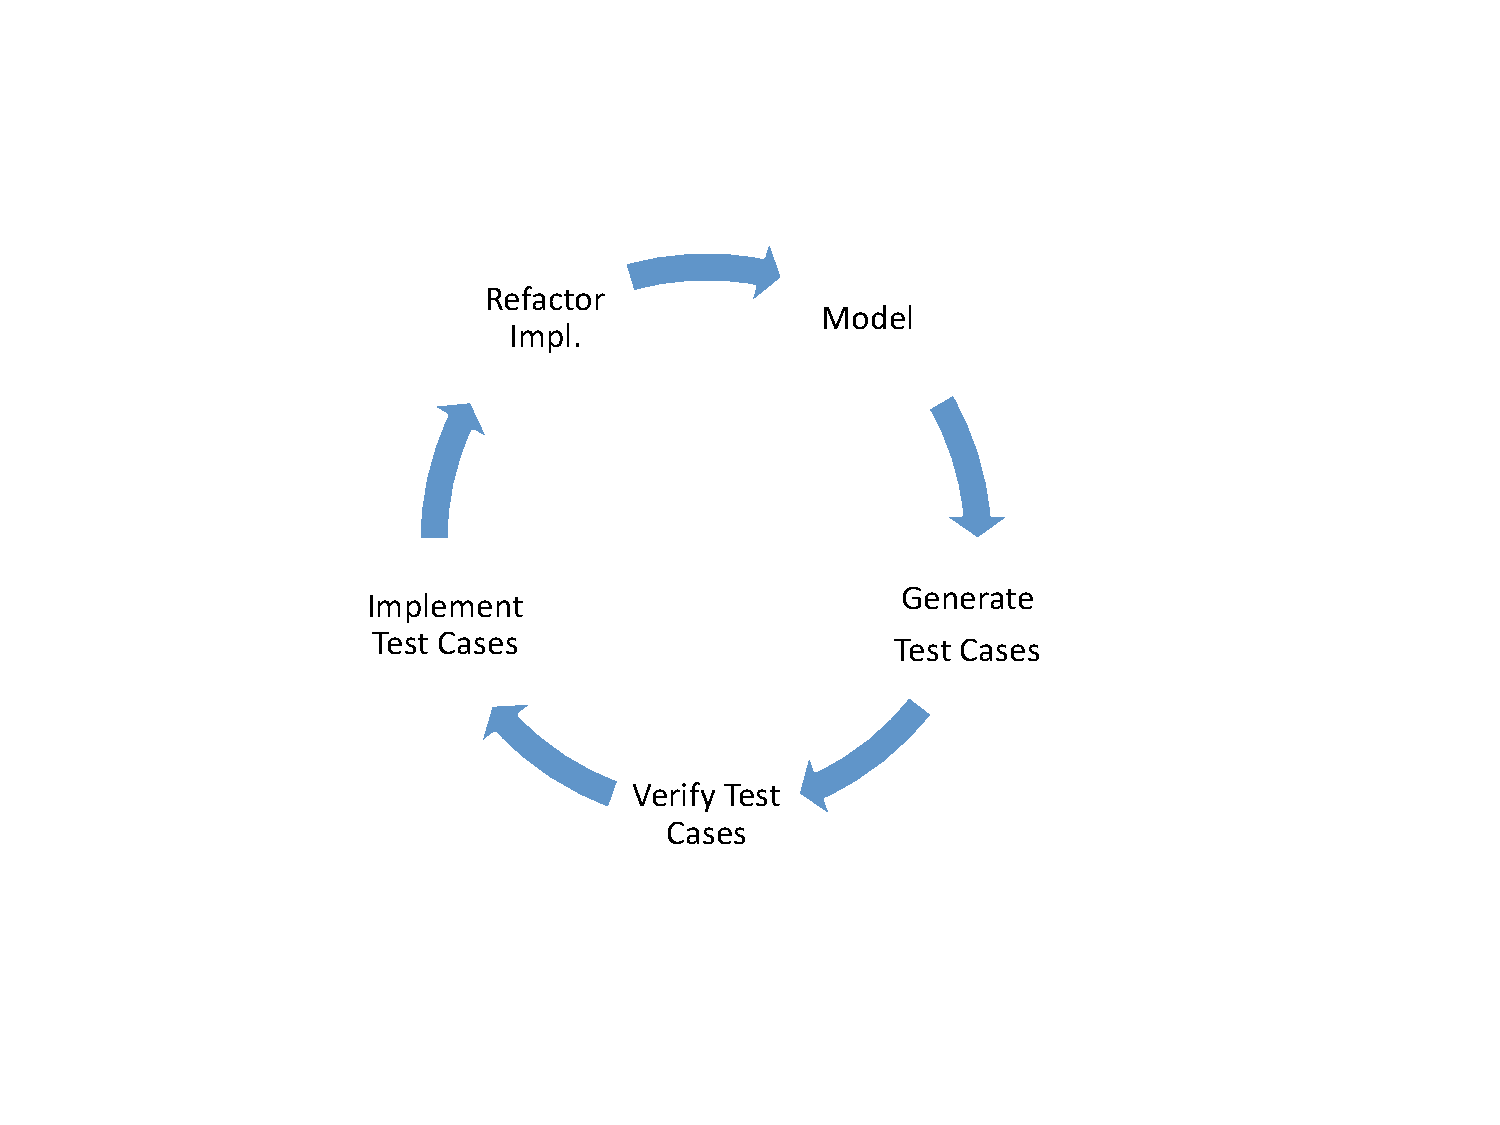
\includegraphics{figures/cycle}
}
\end{minipage}
\end{frame}

%%%%%%%%%%%%%%%%%%%%%%%%%%%%%%%%%%%%%%%%%%%%%%%%%%%%%%%%%%%%%%%%%%%%%%%%%%%%
\section{Bonus}
%%%%%%%%%%%%%%%%%%%%%%%%%%%%%%%%%%%%%%%%%%%%%%%%%%%%%%%%%%%%%%%%%%%%%%%%%%%%


\begin{frame}[fragile]
   \frametitle{OOAS: Type And Variable Definitions}
   \Lsta
\end{frame}

\begin{frame}[fragile]
   \frametitle{OOAS: Input Actions}
   \Lstb
   ...
\end{frame}

\begin{frame}[fragile]
   \frametitle{OOAS: Output Actions}
   \Lstc
\end{frame}

\begin{frame}[fragile]
   \frametitle{OOAS: Protocol Layer}
   \Lstd
\end{frame}



%%%%%%%%%%%%%%%%%%%%%%%%%%%%%%%%%%%%%%%%%%%%%%%%%%%%%%%%%%%%%%%%%%%%%%%%%%%%
\end{document}
%%%%%%%%%%%%%%%%%%%%%%%%%%%%%%%%%%%%%%%%%%%%%%%%%%%%%%%%%%%%%%%%%%%%%%%%%%%%

%% EOF
